%%%%%%%%%%%%%%%%%%%%%%%%%%%%%%%%%%%%%%%%%
% Masters/Doctoral Thesis
%
% %%%%% IMPORTANT %%%%%
% 1) Edit Front/vars.tex
% 2) Compile Front/main.tex
% 3) Edit vars.tex
% 4) Edit precontent.tex
%
% BEFORE ANYTHING ELSE
% You can also set some interesting stuff in the preamble.tex file
% If you know what you're doing.
%%%%%%%%%%%%%%%%%%%%%%%%%%%%%%%%%%%%%%%%%

% The default font size and two-sided printing
% For a one-sided printing change the flag "twoside" to "oneside"
\documentclass[11pt, oneside, table,xcdraw]{Thesis}


%-------------------------------------------------------------------------
%   PREAMBLE AND SETTINGS
%-------------------------------------------------------------------------
% Add the preamble. You can change various settings in here
%-------------------------------------------------------------------------
%	PACKAGES AND OTHER DOCUMENT CONFIGURATIONS
%-------------------------------------------------------------------------

% Include pdf pages in the document
% Necessary to include the front pages (cover and etc.)
\usepackage{pdfpages}

% For the cover page
\usepackage{tikz}

% Fix top page geometry on long titles
\setlength{\headheight}{14pt}  %Try fix error

% Language hyphenation and typographical rules
\usepackage[portuguese,english]{babel}
%Custom hyphenization
\hyphenation{Py-thon}
\hyphenation{Ju-py-ter}
\hyphenation{Ma-the-ma-ti-ca}

% Inline quotes
% added for \begin{displayquote}
\usepackage[autostyle]{csquotes}

% Bibliography setup
% Use the natbib reference package - read up on this to edit the reference
% style; if you want text (e.g. Smith et al., 2012) for the in-text references
% (instead of numbers), remove 'numbers'
\usepackage[square, numbers, comma, sort&compress]{natbib}
\bibliographystyle{IEEEtranN}  % I actually quite like this one
% \bibliographystyle{apsrev4-1-etal} % With emphasized titles. ORIGINAL
% Prevent that the first citation is in the ToC
\usepackage{notoccite}
\setlocalecaption{english}{bib}{References}

% Interesting float placements (like 'H') and custom float types
\usepackage{float}
% Text wrapped around pictures
% https://pt.sharelatex.com/learn/Wrapping_text_around_figures
\usepackage{wrapfig}
% Force float barriers, use as \FloatBarrier
\usepackage[section]{placeins}
% Place floats *above* footnotes
\usepackage[bottom, perpage, symbol]{footmisc}
\renewcommand{\thefootnote}{\arabic{footnote}}
% Set default float placement
\makeatletter
\renewcommand{\fps@figure}{tbph}
\renewcommand{\fps@table}{tbph}
\makeatother

% Pretty colours
\usepackage{xcolor}
% \usepackage{color} % Deprecated by xcolor

% SVGs with Inkscape and PDF+LaTeX
% https://tex.stackexchange.com/questions/473994/svg-and-inkscape
\usepackage[inkscapearea=page]{svg}
% Specifies the directory where vector are stored
\svgpath{{Svgs/}{svg-inkscape/}}

% Graphics stuff
\usepackage{graphicx}  % invoked by svg
% Specifies the directory where pictures are stored
\graphicspath{{Figures/}}

% For sub-figures and stuff
\usepackage{caption}
\usepackage{subcaption}

% Math stuff
\usepackage{amsmath} % Interesting environments
\usepackage{bm}
\usepackage{amssymb} % Interesting symbols
\usepackage{commath} % Interesting macros
\usepackage{braket} % Dirac bra-ket and set notations
%\usepackage{mathpazo} % Math font (palatino for Computer Modern on math)
\usepackage{lmodern}
\usepackage{mathtools} % Mathematical tools to use with amsmath
\setstretch{1.5}
% Math alphabet
\DeclareMathAlphabet{\pazocal}{OMS}{zplm}{m}{n}
\newcommand{\Sa}{\pazocal{S}}
\newcommand{\Ua}{\pazocal{U}}
\newcommand{\Ha}{\pazocal{H}}
\newcommand{\Fa}{\pazocal{F}}
\newcommand{\Ia}{\pazocal{I}}
\newcommand{\Ea}{\pazocal{E}}
\newcommand{\ja}{\pazocal{J}}
%Custom math operators
\DeclareMathOperator*{\meshgrid}{meshgrid}
% Floor and ceiling of numbers
\DeclarePairedDelimiter\ceil{\lceil}{\rceil}
\DeclarePairedDelimiter\floor{\lfloor}{\rfloor}
% Notation variables
\newcommand{\dd}{\mathrm{d}}

% Units and numbers in text
\usepackage{siunitx}
\DeclareSIUnit\baud{Bd} % Baud

% Reimplementation of and extensions to LaTeX verbatim
\usepackage{verbatim} %added for \begin{comment}

% Fancy chapter start quotes
\usepackage{epigraph, varwidth}
% Overload epigraph command
\renewcommand{\epigraphsize}{\small}
\setlength{\epigraphwidth}{0.90\textwidth}
\renewcommand{\textflush}{flushright}
\renewcommand{\sourceflush}{flushright}
% A useful addition
\newcommand{\epitextfont}{\itshape}
\newcommand{\episourcefont}{\scshape}
\makeatletter
\newsavebox{\epi@textbox}
\newsavebox{\epi@sourcebox}
\newlength\epi@finalwidth
\renewcommand{\epigraph}[2]{%
  \vspace{\beforeepigraphskip}
  {\epigraphsize\begin{\epigraphflush}
   \epi@finalwidth=\z@
   \sbox\epi@textbox{%
     \varwidth{\epigraphwidth}
     \begin{\textflush}\epitextfont#1\end{\textflush}
     \endvarwidth
   }%
   \epi@finalwidth=\wd\epi@textbox
   \sbox\epi@sourcebox{%
     \varwidth{\epigraphwidth}
     \begin{\sourceflush}\episourcefont#2\end{\sourceflush}%
     \endvarwidth
   }%
   \ifdim\wd\epi@sourcebox>\epi@finalwidth
     \epi@finalwidth=\wd\epi@sourcebox
   \fi
   \leavevmode\vbox{
     \hb@xt@\epi@finalwidth{\hfil\box\epi@textbox}
     \vskip1.75ex
     \hrule height \epigraphrule
     \vskip.75ex
     \hb@xt@\epi@finalwidth{\hfil\box\epi@sourcebox}
   }%
   \end{\epigraphflush}
   \vspace{\afterepigraphskip}}}
\makeatother
%End of overload command


% Use more than one optional parameter in a new commands
\usepackage{xargs}

\usepackage{transparent}

% Code listings
\usepackage{listings}
% Colors for the listing
\definecolor{dkgreen}{rgb}{0,0.6,0}
\definecolor{gray}{rgb}{0.5,0.5,0.5}
\definecolor{mauve}{rgb}{0.58,0,0.82}
\definecolor{codegreen}{rgb}{0,0.6,0}
\definecolor{codegray}{rgb}{0.5,0.5,0.5}
\definecolor{codepurple}{rgb}{0.58,0,0.82}
\definecolor{backcolour}{rgb}{0.95,0.95,0.92}
\definecolor{orange}{RGB}{255,127,0}
% Python style for code blocks
\lstdefinestyle{Python}{
        language=Python,
         numberstyle=\small,
         stepnumber=2,
         numbersep=10pt,
         basicstyle={\small\ttfamily},
         keywordstyle    = \color{blue},
         commentstyle    = \color{red}\ttfamily,
         stringstyle=\color{orange},
         tabsize=2,
         columns=fullflexible,
         backgroundcolor=\color{backcolour},
         frame=none,
         numbers=left,
         aboveskip=5mm,
         belowskip=5mm,
         breaklines=true
}

% Algorithmicx provides a flexible, yet easy to use, way for inserting good
% looking pseudocode or source code in your papers.
\usepackage{algorithmicx}

% Hyperref and Backref
% backref makes the bibliography say where the entry was cited.
% For the print version of the thesis you might wanna set all colors to back
\usepackage{hyperref}
\usepackage[hyperpageref]{backref}
\hypersetup{colorlinks, citecolor=black, urlcolor=black,
        linkcolor=black, breaklinks=true, hypertexnames=true}
\renewcommand*{\backref}[1]{}
\renewcommand*{\backrefalt}[4]{%
    \ifcase #1%
          \or [Cited on page~#2.]%
          \else [Cited on pages~#2.]%
    \fi%
    }
\usepackage{cleveref}
    
% Interesting URL breakings
\usepackage{url}
\def\UrlBreaks{\do\/\do-\do\&\do.\do:}

% Variants of \fbox and other games with boxes
\usepackage{fancybox}

% LaTeX default text is fully-justified, but often left-justified text may be a
% more suitable format. This left-alignment can be easily accomplished by
% importing the ragged2e package.
\usepackage{ragged2e}

% Create tabular cells spanning multiple rows
\usepackage{multirow}

% Changes bullet points marker
\renewcommand{\labelitemi}{\(\bullet\)}

% Notes on the documents
% https://tex.stackexchange.com/questions/9796/how-to-add-todo-notes
% https://tex.stackexchange.com/questions/316220/todo-commentsnot-include-and-left-align
% Examples:
% \unsure{Is this correct?}, \change{Change this!},
% \info{This can help me in chapter seven!}
% \improvement{This really needs to be improved!\\ What was I thinking?!}
% \thiswillnotshow{This is hidden since option `disable' is chosen!}
% WARNING: It eliminates whitespaces in front of it.
% You can add trailing {} to avoid.

\usepackage[colorinlistoftodos,
    prependcaption,
    textsize=tiny,
    textwidth=2cm]
        {todonotes}
% You can add:
% \setlength{\marginparwidth}{3cm}\reversemarginpar
% before \todo on each command for a different effect
\newcommandx{\unsure}[2][1=]{
    % \setlength{\marginparwidth}{3cm}\reversemarginpar
    \todo[linecolor=red,backgroundcolor=red!25,bordercolor=red,#1]{#2}
    }
\newcommandx{\change}[2][1=]{
    % \setlength{\marginparwidth}{3cm}\reversemarginpar
    \todo[linecolor=blue,backgroundcolor=blue!25,bordercolor=blue,#1]{#2}
    }
\newcommandx{\info}[2][1=]{
    % \setlength{\marginparwidth}{3cm}\reversemarginpar
    \todo[linecolor=green,backgroundcolor=green!25,bordercolor=green,#1]{#2}
    }
\newcommandx{\improvement}[2][1=]{
    % \setlength{\marginparwidth}{3cm}\reversemarginpar
    \todo[linecolor=yellow,backgroundcolor=yellow!25,bordercolor=yellow,#1]{#2}
    }
\newcommandx{\thiswillnotshow}[2][1=]{\todo[disable,#1]{#2}}

% Use Arial as main font
% Need to use the LuaLaTex compiler
\usepackage{fontspec}
\setmainfont{Arial}

\usepackage[acronym,toc,shortcuts]{glossaries}
\makeglossaries
%\usepackage{acronym} 

% \usepackage{tocloft}

% \renewcommand{\cftchapaftersnum}{.}%
% \renewcommand{\cftsecaftersnum}{.}%
% \renewcommand{\cftsubsecaftersnum}{.}%
% \renewcommand{\cftsubsubsecaftersnum}{.}%

%\usepackage{titletoc}
\usepackage[dotinlabels]{titletoc}
\contentsmargin{0em}


\dottedcontents{section}[3.9em]{}{2.3em}{3pt}
\dottedcontents{subsection}[84pt]{}{3.2em}{3pt}
\dottedcontents{subsubsection}[104pt]{}{4.0em}{3pt}
\dottedcontents{chapter}[20pt]{}{20pt}{3pt}
\dottedcontents{figure}[20pt]{}{20pt}{3pt}
\dottedcontents{table}[20pt]{}{20pt}{3pt}

%https://tex.stackexchange.com/questions/493343/add-dotted-lines-in-toc-without-changing-spacing


%\renewcommand{\cftchapaftersnum}{.}%

\usepackage{caption}
\captionsetup{justification=raggedright,singlelinecheck=false}

\setcounter{secnumdepth}{3}
\setcounter{tocdepth}{3}
% \usepackage{tocloft}%


\titleformat{\subsection}  % which section command to format
  {\fontsize{12}{14}} % format for whole line
  {\thesubsection} % how to show number
  {1em} % space between number and text
  {} % formatting for just the text
  [] % formatting for after the text

\titlespacing\chapter{0pt}{12pt plus 4pt minus 2pt}{0pt plus 2pt minus 2pt}
\titlespacing\section{0pt}{12pt plus 4pt minus 2pt}{0pt plus 2pt minus 2pt}
\titlespacing\subsection{0pt}{12pt plus 4pt minus 2pt}{0pt plus 2pt minus 2pt}
\titlespacing\subsubsection{0pt}{12pt plus 4pt minus 2pt}{0pt plus 2pt minus 2pt}



% Thesis settings. THIS IS VERY IMPORTANT YOU CHANGE
% !TEX root = main.tex

%-------------------------------------------------------------------------
%	PARAMETERS FOR FCUP THESIS TITLEPAGES/BOOK COVER
%-------------------------------------------------------------------------

% THESIS TYPEs:
% - msc (Master of Sciences)
% - phd (Doctor of Philosophy)
\thesistype{msc}

% Book spine width (CAREFUL: MIN 8mm)
\spinewidth{10mm}

% Thesis front title
\fronttitle{Modified gravity from the viewpoint of backreaction}

% Front title spacing multiplier
% NOTE: you may want to adjust this value to 1.15/1.20 after changing to your
% thesis title
\titlespacing{1.15}

% Book spine title
\spinetitle{Modified gravity from the viewpoint of backreaction}

% Author name
\authorname[mailto:up202203990@fc.up.pt]{Bruno Francisco Parracho}

% Affiliation number 2
% USAGE: \otheraffiliation[url]{relative/path/to/logo}{INITIAL}{University name}
%\otheraffiliation[http://uni2.pt]{logos/logo2}{UNI2}{Universidade/Faculdade 2}

% Affiliation number 3
% USAGE: \extraaffiliation[url]{relative/path/to/logo}{INITIAL}{University name}
%\extraaffiliation[http://uni3.pt]{logos/logo3}{UNI3}{Universidade/Faculdade 3}

% Degree name
\degreename{Mestrado em Física}

% Field of science
\sciencefield{Física}

% Department name
\department[http://dfa.fc.up.pt/]{Departamento de Física e Astronomia}

% Supervisor info
% Supervisor name
\supervisor[mailto:jpmimoso@fc.ul.pt]{Prof. Dr. José Pedro Mimoso}
% Supervisor name position/Category (comment out to hide this field)
%\supervisorposition{Categoria} %
% Supervisor university/faculty
\supervisoraffiliation[]{Faculdade de Ciências da Universidade de Lisboa}
% Supervisor secondary affiliation
\supervisoraffiliation[]{Instituto de Astrofísica e Ciências do Espaço}

% Cosupervisor info ----- Comment out if not needed
% Cosupervisor name
\cosupervisor[mailto:ppavelin@fc.up.pt]{Prof. Dr. Pedro Avelino}
% Cosupervisor name position/Category (comment out to hide this field)
%\cosupervisorposition{Categoria}
% Supervisor university/faculty
\cosupervisoraffiliation[]{Faculdade de Ciências da Universidade do Porto}
\cosupervisoraffiliation[]{Instituto de Astrofísica e Ciências do Espaço}

% ------------------


%-------------------------------------------------------------------------
%	DOCUMENT
%-------------------------------------------------------------------------

\begin{document}

% Start counting pages in an unused scheme to fix backref
\pagenumbering{Alph}

% Includes the front pages (cover and etc.)
%\pagestyle{empty}
%
\includepdf[pages={1},pagecommand={},scale=1]{Front/Cover/template}
%\cleardoublepage
%
\includepdf[pages={2},pagecommand={},scale=1]{Front/Cover/template}
%\cleardoublepage
\pagestyle{fancy}

%----------- Failed attempt to make cover page in latex ------------------

% Cover page
%\newgeometry{bindingoffset=0cm,
%	top=1.27cm,
%	outer=1.27cm,
%	inner=1.27cm,
%	bottom=1.27cm}

%\pagestyle{empty}
%
%\begin{picture}(-5,0)(2.5,0)
%% MSc symbol
%\put(331.8,-808.061){
\includegraphics[width=267.6pt,height=464.25pt]{Front/Cover/MSc.png}}
%% FEUP logo
%\put(382,-345){
\includegraphics[width=155.9pt]{Front/Cover/FEUP.png}}
%% FCUP logo
%\put(360.5,-293){
\includegraphics[width=183pt]{Front/logos/fcup.png}}
%\end{picture}
%
%%\makebox[12cm][l]{\ttitle}
%
%\vfill
%\parbox[t][12cm][t]{12cm}{\bf\fontsize{55}{0}\selectfont\ttitle}
%\vfill
%
%\restoregeometry

%-------------------------------------------------------------------------

% Use roman page numbering style (i, ii, iii, iv...) for the pre-content pages
\frontmatter

% Title page
%\maketitle

% Edit this file!

%-------------------------------------------------------------------------
%	QUOTATION PAGE
%-------------------------------------------------------------------------
%\quotepage{Matt Smith as \emph{The Doctor}, written by Matthew Graham}
%{
%	I am and always will be the optimist, the hoper of far-flung hopes and the
%	dreamer of \newline improbable dreams
%}

%-------------------------------------------------------------------------
%	DEDICATORY
%-------------------------------------------------------------------------

%\begin{dedicatory}
%	Dedicated to (optional) 
%\end{dedicatory}

%-------------------------------------------------------------------------
%	ACKNOWLEDGEMENTS PAGE
%-------------------------------------------------------------------------
\addtocontents{toc}{\protect\setcounter{tocdepth}{-1}}
\begin{acknowledgements}

Acknowledge ALL the people!

\end{acknowledgements}
\addtocontents{toc}{\protect\setcounter{tocdepth}{3}}
%\addvspacetoc{0.3cm} % Add a gap in the Contents, for aesthetics


%-------------------------------------------------------------------------
%	ABSTRACT PAGE (PORTUGUESE)
%-------------------------------------------------------------------------
\addtocontents{toc}{\protect\setcounter{tocdepth}{-1}}
\begin{abstract}[
	thesistitle={Gravitação Modificada do ponto de vista de retroaação},
	title={Resumo},
	degree={Mestrado em Física},
	nameconnector={por},
        keywordsname={Palavras-chave},
        keywords={física (keywords em português)}]
\begin{otherlanguage}{portuguese}

Este tese é sobre alguma coisa



\end{otherlanguage}
\end{abstract}
\addtocontents{toc}{\protect\setcounter{tocdepth}{3}}
%-------------------------------------------------------------------------
%	ABSTRACT PAGE
%-------------------------------------------------------------------------
\addtocontents{toc}{\protect\setcounter{tocdepth}{-1}}
\begin{abstract}

This thesis is about something, I guess.

\end{abstract}
\addtocontents{toc}{\protect\setcounter{tocdepth}{3}}

%-------------------------------------------------------------------------
%	LIST OF CONTENTS/FIGURES/TABLES
%-------------------------------------------------------------------------

\addtocontents{toc}{\protect\setcounter{tocdepth}{-1}}

\tableofcontents % Write out the Table of Contents

\addtocontents{toc}{\protect\setcounter{tocdepth}{3}}
\addvspacetoc{0.3cm}

%\listoftables % Write out the List of Tables

\listoffigures % Write out the List of Figures



%\addvspacetoc{0.3cm}

%-------------------------------------------------------------------------
%	PHYSICAL CONSTANTS/OTHER DEFINITIONS
%-------------------------------------------------------------------------

%\begin{listofcontants}
%	\const{My little ponny test of magical rainbow}{$mn/mp$}
%    {$2.997\ 924\ 58\times10^{8}\ \mbox{ms}^{-\mbox{s}}$}
%   \const{Vaccuum permeability test of magical rainbow for a specific case of
%   condensed matter physics}
%   {$\epsilon_0$}{$2.997\ 924\ 58\times10^{8}\ \mbox{ms}^{-\mbox{s}}$}
%	\const{Speed of Light test of magical rainbow}{$c$}
%    {$2.997\ 924\ 58\times10^{8}\ \mbox{ms}^{-\mbox{s}}$}
%\end{listofcontants}


%-------------------------------------------------------------------------
%	SYMBOLS
%-------------------------------------------------------------------------

%\begin{listofsymbols}
%	\symb{$F_{\mu\nu}$}{Maxwell tensor}{F}
%	\symb{$a$}{distance}{m}
%	\\
%	\symb{$\omega$}{angular frequency}{rads$^{-1}$}
%\end{listofsymbols}


%-------------------------------------------------------------------------
%	NOTATION
%-------------------------------------------------------------------------

% \newcommand\notationname{Notation and Conventions}
% \addtotoc{\notationname}
% \fancyhead[LO]{\textsc{\notationname}}

% \input{Notation}



%-------------------------------------------------------------------------
%	ABBREVIATIONS
%-------------------------------------------------------------------------

\newacronym{ann}{ANN}{Artificial Neural Network}

\printglossary[type=\acronymtype,title={List of Abbreviations}]



%-------------------------------------------------------------------------
%	THESIS CONTENT - CHAPTERS
%-------------------------------------------------------------------------

\addvspacetoc{0.3cm}

% Begin numeric (1,2,3...) page numbering
\mainmatter

\pagestyle{fancy}
\renewcommand{\chaptermark}[1]{\markboth{\thechapter. \textsc{#1}}{}}
%\fancyhead[LO]{\leftmark}


%%% -----------  ADD CHAPTERS HERE ------------------ %%%

\chapter{Introduction}







\section{}



\section{Structure outline}

The first chapter of this work, this introduction, aims to establish the scene for the following content and to give an overview of the subject.

In the second chapter we first study the $3+1$ covariant formalism. This formalism creates the framework through which the spacetime manifold can be decomposed into a slicing of spacelike hypersurfaces, each perpendicular to a chosen timelike vector. Secondly, we check the conformal counterparts of the dynamical quantities of the formalism.

The third chapter is to present a general covariant and gauge invariant averaging procedure applied to the past light-cone of an observer and to introduce the correspoding Buchert-Ehlers commutation rules. 

The fourth chapter is dedicated to the study and discussion of modified theories of gravity, mainly Brans-Dicke theories, where we introduce a new scalar field, the Brans-dicke fluid.

The fifth chapter is devoted initially to present the general Buchert equations, where we underline the various types of backreaction, followed by applying the previously obtained formalisms and averaging procedure to the Brans-Dicke theory, in order to determine the equivalent Friedmann equations.


\section{Notation and conventions}
\begin{itemize}
    \item Spacetime indices are represented by Greek letters and adquire values from 0 to 3, i.e. $\mu,\nu,\lambda,\ldots - 0,1,2,3$.
    \item Spatial indices are indicated by Latin letters starting from $i$ onwards and run from 1 to 3, i.e. $i,j,k,\ldots - 1,2,3$.
%    \item Angular indices are shown by Latin letter starting from $a$ until $g$ and run from 2 to 3, i.e. $a,b,c,\ldots - 2,3$.
    \item Einstein summation convenction is used: repeated index implies summation over all the possible values of the index.
    \item Quantities in bold denote tensor and vector fields without writing indeces, e.g. $\mathbf{u},\mathbf{h},\mathbf{K},\prescript{3}{}{\mathbf{R}}$.
    \item The signature of the metric is $(-,+,+,+)$.
    \item Natural units are employed, to the extent that $c=1$.
    \item Equality by definition is indicated by $:=$.
    \item Equality by algebraic identity is represented by $\equiv$.
    \item Symmetrization is represented by round brackets, for example: $T_{(\mu\nu)}:=\frac{1}{2}(T_{\mu\nu}+T_{\nu\mu})$.
    \item Antisymmetrization is represented by square brackets, for example: $T_{[\mu\nu]}:=\frac{1}{2}(T_{\mu\nu}-T_{\nu\mu})$.
    \item Traceless tensors are represented by angle brackets, for example: $T_{\langle\mu\nu\rangle}:=T_{(\mu\nu)}-\frac{1}{3}g_{\mu\nu}(g^{\lambda\rho}T_{\lambda\rho})$.
    \item The partial derivative w.r.t $x^\mu$ is indicated by $\partial_\mu$ or with a comma, for example: $u_{\mu,\nu}=\partial_\nu u_\mu$.
    \item The covariant derivative w.r.t $x^\mu$ is indicated by $\nabla_\mu$ or with a semicolon, for example: $u_{\mu;\nu}=\nabla_\nu u_\mu$.
\end{itemize}
\chapter{3+1 Formalism}

The 3+1 formalism is a method in general relativity, where we slice the spacetime manifold into a foliation of Cauchy hypersurfaces (three-dimensional surfaces). 
Due to the metric induced by the Lorentzian spacetime metric needing to be Riemannian, the hypersurfaces are required to be spacelike.
From a naïve point of view, this can be seen as a decomposition from spacetime into "space" + "time". It should be noted this spliting requires a well established and concise choice of time coordinate.

This formalism is also useful for solving the initial value problem, with this decomposition, solving the Einstein equation is equivalent to solving a Cauchy problem.

Studies with the 3+1 formalism started in the 1920s by Georges Darmois and continued until the 1950s, by direct affiliations. In 1952, Yvonne Choquet-Bruhat verified that the Cauchy problem, arising from the 3+1 decomposition has locally a unique solution \cite{}.
Later in the decade, Dirac motivated a similar formalism, based on an Hamiltonian approach, which later was called ADM, by Arnowitt, Deser and Misner\cite{}. Around the same time, Wheeler introduced the concept of geometrodynamics and coined the terms, soon mentioned, "lapse" and "shift". 
In the 1970s, the 3+1 formalism became an essential tool, to numerical relativity.

In this chapter, we will be only considering a single general fluid.

\section{Description of the geometry}

Let us consider a four-dimensional manifold, $\mathcal{M}$, with a Lorentzian metric tensor $\mathbf{g}$ and described under a local coordinate system $x^\mu=(y,x^i)$, where $\mathbf{g}=g_{\mu\nu}dx^\mu \otimes dx^\nu$. 
In this spacetime, matter is described by a matter content fluid, where the fluid flow is described by a timelike congruence with a unit, future-oriented, timelike tangent four-vector field $\mathbf{u}$, describing its four-velocity. 
Meanwhile we will not make any exact physical interpretation on this four-velocity\footnote{The four-velocity could be a energy frame of the fluid, a barycentric velocity, or the unit vector associated to another conserved current.}.

The foliation is performed by slicing $\mathcal{M}$ in a family $y=\text{const}$ hypersurfaces which we denote $\Sigma_y$. 
Locally these hypersurfaces will share the same topology $\Sigma_y \simeq \Sigma$. 
Therefore locally we have $\mathcal{M}\simeq \mathbb{R}\times \Sigma$. 
And we denote by $\mathbf{n}$ their unit, future-oriented and timelike normal vector field, which generally is tilted with respect to the four-velocity $\mathbf{u}$.
And we denote by $\bm{\partial_y}$ the vector parallel to the motion along $y$, when the $x^i$ are held fixed.
We can characterize this foliation by a scalar function $y$ restrictively increasing along each flow line, and defined in such a way that each hypersurface is a level set of $y$. For the time being we choose the time coordinate $t$, as this stricly increasing function, implying that $y\equiv y(t)$. 


\begin{figure}[ht]
    \centering

\tikzset{every picture/.style={line width=0.75pt}} %set default line width to 0.75pt        

\begin{tikzpicture}[x=0.75pt,y=0.75pt,yscale=-1,xscale=1]
%uncomment if require: \path (0,467); %set diagram left start at 0, and has height of 467

%Curve Lines [id:da13576815661454944] 
\draw [color={rgb, 255:red, 22; green, 144; blue, 36 }  ,draw opacity=1 ]   (48,205.36) .. controls (81,292.72) and (97.5,291.16) .. (206.12,352) ;
%Curve Lines [id:da3389506239015292] 
\draw [color={rgb, 255:red, 22; green, 144; blue, 36 }  ,draw opacity=1 ]   (206.12,352) .. controls (273.5,342.64) and (285.88,342.64) .. (358.75,347.32) .. controls (431.63,352) and (457.75,347.32) .. (510,331.72) ;
%Curve Lines [id:da2722842924714688] 
\draw [color={rgb, 255:red, 22; green, 144; blue, 36 }  ,draw opacity=1 ]   (347.75,196) .. controls (378,228.76) and (389,214.72) .. (435.75,244.36) .. controls (482.5,274) and (496.25,311.44) .. (510,331.72) ;
%Curve Lines [id:da2654170172814696] 
\draw [color={rgb, 255:red, 22; green, 144; blue, 36 }  ,draw opacity=1 ]   (48,205.36) .. controls (89.25,222.52) and (98.88,242.8) .. (347.75,196) ;

%Curve Lines [id:da188980808953499] 
\draw [line width=1.5]    (204.9,272.49) .. controls (260.93,275.27) and (284.28,273.88) .. (346.54,261.35) ;
%Curve Lines [id:da33296466436615946] 
\draw  [dash pattern={on 4.5pt off 4.5pt}]  (223.57,283.63) .. controls (279.61,286.41) and (302.96,285.02) .. (365.22,272.49) ;
%Curve Lines [id:da646227828934764] 
\draw  [dash pattern={on 4.5pt off 4.5pt}]  (214.23,278.06) .. controls (270.27,280.84) and (293.62,279.45) .. (355.88,266.92) ;
%Curve Lines [id:da6452967318047047] 
\draw  [dash pattern={on 4.5pt off 4.5pt}]  (267.16,258.57) .. controls (284.28,261.35) and (307.63,280.84) .. (343.43,296.16) ;
%Curve Lines [id:da5657790292060159] 
\draw  [dash pattern={on 4.5pt off 4.5pt}]  (251.59,259.96) .. controls (268.71,262.75) and (292.06,282.24) .. (327.86,297.55) ;
%Curve Lines [id:da9932195493480838] 
\draw [line width=1.5]    (237.58,261.35) .. controls (254.7,264.14) and (278.05,283.63) .. (313.85,298.94) ;
%Curve Lines [id:da056229993422925784] 
\draw  [dash pattern={on 4.5pt off 4.5pt}]  (223.57,262.75) .. controls (240.7,265.53) and (264.04,285.02) .. (299.84,300.33) ;
%Curve Lines [id:da8916754691070794] 
\draw  [dash pattern={on 4.5pt off 4.5pt}]  (209.57,262.75) .. controls (226.69,265.53) and (250.03,285.02) .. (285.83,300.33) ;
%Curve Lines [id:da7913518320312014] 
\draw [color={rgb, 255:red, 22; green, 144; blue, 36 }  ,draw opacity=1 ]   (140,90.36) .. controls (173,177.72) and (189.5,176.16) .. (298.12,237) ;
%Curve Lines [id:da20504120863374542] 
\draw [color={rgb, 255:red, 22; green, 144; blue, 36 }  ,draw opacity=1 ]   (298.12,237) .. controls (365.5,227.64) and (377.88,227.64) .. (450.75,232.32) .. controls (523.63,237) and (549.75,232.32) .. (602,216.72) ;
%Curve Lines [id:da1649144687038906] 
\draw [color={rgb, 255:red, 22; green, 144; blue, 36 }  ,draw opacity=1 ]   (439.75,81) .. controls (470,113.76) and (481,99.72) .. (527.75,129.36) .. controls (574.5,159) and (588.25,196.44) .. (602,216.72) ;
%Curve Lines [id:da3627403092518948] 
\draw [color={rgb, 255:red, 22; green, 144; blue, 36 }  ,draw opacity=1 ]   (140,90.36) .. controls (181.25,107.52) and (190.88,127.8) .. (439.75,81) ;

%Curve Lines [id:da49174619234774997] 
\draw [line width=1.5]    (454,188) .. controls (490,190) and (505,189) .. (545,180) ;
%Curve Lines [id:da12379144432369049] 
\draw  [dash pattern={on 4.5pt off 4.5pt}]  (476,200) .. controls (512,202) and (522,201) .. (562,192) ;
%Curve Lines [id:da34708713312407835] 
\draw  [dash pattern={on 4.5pt off 4.5pt}]  (466,196) .. controls (502,198) and (517,197) .. (557,188) ;
%Curve Lines [id:da6530457587293368] 
\draw  [dash pattern={on 4.5pt off 4.5pt}]  (460,192) .. controls (496,194) and (511,193) .. (551,184) ;
%Curve Lines [id:da9798134589250638] 
\draw  [dash pattern={on 4.5pt off 4.5pt}]  (447,184) .. controls (483,186) and (498,185) .. (538,176) ;
%Curve Lines [id:da8730255973163852] 
\draw  [dash pattern={on 4.5pt off 4.5pt}]  (513,174) .. controls (524,176) and (539,190) .. (562,201) ;
%Curve Lines [id:da1477712395132038] 
\draw  [dash pattern={on 4.5pt off 4.5pt}]  (503,176) .. controls (514,178) and (529,192) .. (552,203) ;
%Curve Lines [id:da49150127520573017] 
\draw  [dash pattern={on 4.5pt off 4.5pt}]  (494,178) .. controls (505,180) and (520,194) .. (543,205) ;
%Curve Lines [id:da641044614887526] 
\draw  [dash pattern={on 4.5pt off 4.5pt}]  (484,179) .. controls (495,181) and (510,195) .. (533,206) ;
%Curve Lines [id:da6160774549922841] 
\draw [line width=1.5]    (475,180) .. controls (486,182) and (501,196) .. (524,207) ;
%Curve Lines [id:da9152067694355859] 
\draw  [dash pattern={on 4.5pt off 4.5pt}]  (466,181) .. controls (477,183) and (492,197) .. (515,208) ;
%Curve Lines [id:da9953141851318603] 
\draw  [dash pattern={on 4.5pt off 4.5pt}]  (457,181) .. controls (468,183) and (483,197) .. (506,208) ;
%Curve Lines [id:da17562105900218739] 
\draw  [dash pattern={on 4.5pt off 4.5pt}]  (447,181) .. controls (458,183) and (473,197) .. (496,208) ;
%Curve Lines [id:da13502174858158433] 
\draw  [dash pattern={on 0.84pt off 2.51pt}]  (140,384) .. controls (170,261) and (566,192) .. (609,123) ;
%Straight Lines [id:da39979917949234345] 
\draw    (265,274) -- (265,188) ;
\draw [shift={(265,186)}, rotate = 90] [color={rgb, 255:red, 0; green, 0; blue, 0 }  ][line width=0.75]    (10.93,-3.29) .. controls (6.95,-1.4) and (3.31,-0.3) .. (0,0) .. controls (3.31,0.3) and (6.95,1.4) .. (10.93,3.29)   ;
%Straight Lines [id:da12059773309792465] 
\draw    (265,274) -- (432.14,206.75) ;
\draw [shift={(434,206)}, rotate = 158.08] [color={rgb, 255:red, 0; green, 0; blue, 0 }  ][line width=0.75]    (10.93,-3.29) .. controls (6.95,-1.4) and (3.31,-0.3) .. (0,0) .. controls (3.31,0.3) and (6.95,1.4) .. (10.93,3.29)   ;
%Straight Lines [id:da5100745631342329] 
\draw    (100,104) ;
%Straight Lines [id:da8476136722912351] 
\draw    (265,274) -- (330.96,165.71) ;
\draw [shift={(332,164)}, rotate = 121.35] [color={rgb, 255:red, 0; green, 0; blue, 0 }  ][line width=0.75]    (10.93,-3.29) .. controls (6.95,-1.4) and (3.31,-0.3) .. (0,0) .. controls (3.31,0.3) and (6.95,1.4) .. (10.93,3.29)   ;
%Straight Lines [id:da18587682422680873] 
\draw  [dash pattern={on 4.5pt off 4.5pt}]  (434,206) -- (434,301) ;
%Straight Lines [id:da09067623901522537] 
\draw    (265,274) -- (431.02,295.74) ;
\draw [shift={(433,296)}, rotate = 187.46] [color={rgb, 255:red, 0; green, 0; blue, 0 }  ][line width=0.75]    (10.93,-3.29) .. controls (6.95,-1.4) and (3.31,-0.3) .. (0,0) .. controls (3.31,0.3) and (6.95,1.4) .. (10.93,3.29)   ;
%Straight Lines [id:da13097975178971488] 
\draw  [dash pattern={on 4.5pt off 4.5pt}]  (332,164) -- (333,234) ;
%Straight Lines [id:da6716736044337814] 
\draw    (265,274) -- (331.28,235.01) ;
\draw [shift={(333,234)}, rotate = 149.53] [color={rgb, 255:red, 0; green, 0; blue, 0 }  ][line width=0.75]    (10.93,-3.29) .. controls (6.95,-1.4) and (3.31,-0.3) .. (0,0) .. controls (3.31,0.3) and (6.95,1.4) .. (10.93,3.29)   ;
%Straight Lines [id:da678571273463811] 
\draw    (333,234) -- (431.3,294.95) ;
\draw [shift={(433,296)}, rotate = 211.8] [color={rgb, 255:red, 0; green, 0; blue, 0 }  ][line width=0.75]    (10.93,-3.29) .. controls (6.95,-1.4) and (3.31,-0.3) .. (0,0) .. controls (3.31,0.3) and (6.95,1.4) .. (10.93,3.29)   ;
%Curve Lines [id:da2413544430582497] 
\draw  [dash pattern={on 0.84pt off 2.51pt}]  (230,359) .. controls (242,303) and (291,207) .. (405,122) ;
%Curve Lines [id:da8442704583638048] 
\draw  [dash pattern={on 0.84pt off 2.51pt}]  (285,424) .. controls (259,320) and (257,264) .. (297,125) ;
%Straight Lines [id:da7592467478741162] 
\draw  [dash pattern={on 4.5pt off 4.5pt}]  (265,186) -- (434,206) ;

% Text Node
\draw (309.69,308.09) node [anchor=north west][inner sep=0.75pt]    {$x^{i}$};
% Text Node
\draw (72,225.4) node [anchor=north west][inner sep=0.75pt]    {$\Sigma _{t}$};
% Text Node
\draw (158,112.4) node [anchor=north west][inner sep=0.75pt]    {$\Sigma _{t+\delta t}$};
% Text Node
\draw (228,173.4) node [anchor=north west][inner sep=0.75pt]    {$N\mathbf{n}$};
% Text Node
\draw (503,141.4) node [anchor=north west][inner sep=0.75pt]    {$C( \partial _{t})$};
% Text Node
\draw (408,181.4) node [anchor=north west][inner sep=0.75pt]    {$\partial _{t}$};
% Text Node
\draw (108,389.4) node [anchor=north west][inner sep=0.75pt]    {$x^{i} =const$};
% Text Node
\draw (299,139.4) node [anchor=north west][inner sep=0.75pt]    {$\frac{N}{\Gamma }\mathbf{u}$};
% Text Node
\draw (351,104.4) node [anchor=north west][inner sep=0.75pt]    {$C( u)$};
% Text Node
\draw (356,296.4) node [anchor=north west][inner sep=0.75pt]    {$\mathbf{\beta }$};
% Text Node
\draw (247,113.4) node [anchor=north west][inner sep=0.75pt]    {$C( n)$};


\end{tikzpicture}
        \caption{Scheme entailing the context of the geometrical quantities: $\mathbf{n}$ normal vector field to the hypersurface; $\mathbf{u}$ the 4-velocity vector field (fluid flow lines) with congruence $C(u)$; $\partial_t$ is the tangent vector to the constant coordinates lines ($x^i=const$) with congruence $C(\partial_t)$ (time-vector of the coordinate basis).}
        \label{fig:foliation}
\end{figure}

Based on the Fig.\ref{fig:foliation} we can write $\mathbf{n}$ as,
\begin{equation}
    \mathbf{n}= \frac{1}{N}(\partial_t-\beta^i\partial_i) \Leftrightarrow n^\mu = \frac{1}{N}(1,-\beta^i)
    \label{eqn:def_normal_vector_upper}
\end{equation}
where $N$, $\beta^i$ are respectively known as the "lapse function" and "shift vector". The components of the corresponding covector $n_\mu$, is given by,
\begin{equation}
    n_\mu=-N(1,0),
    \label{eqn:def_normal_vector_lower}
\end{equation}
where $n^\mu n_\mu=-1$.

The lapse function is a positive valued function and determines how far consecutive slices are from each other, in the time direction of each point in the slice. 
While the shift vector representes the spatial displacement between consecutive slices at the same spatial coordinate point.


In the 3+1 formalism, spacetime tensor are projected onto the hypersurfaces by applying a operator $\mathbf{h}=h_{\mu\nu}dx^\mu\otimes dx^\nu$, some important propeties are,
\begin{equation}
    h_{\mu\nu}:=g_{\mu\nu}+n_\mu n_\nu, \qquad h_{\mu\nu}n^\nu=0, \qquad h^\mu_\lambda h^\lambda_\nu = h^\mu_\nu, \qquad h^{\mu\nu}h_{\mu\nu}=3,
    \label{eqn:h_properties}
\end{equation}
where the spatial component of the projector, $h_{ij}$ is the induced Riemannian metric on the slices. The line element is then decomposed into,
\begin{equation}
    ds^2=g_{\mu\nu}dx^\mu dx^\nu=-N^2dt^2+h_{ij}(dx^i+\beta^i dt)(dx^j+\beta^j dt),
    \label{eqn:general_spacetime_metric}
\end{equation}



\section{Description of the fluid}

\subsection{Decomposition of the fluid velocity}

In the perfect fluid model, matter is represented as a vector $\mathbf{u}$, which is timelike and unitary, $u^\mu u_\mu = -1$. Usually we see it in the energy-momentum tensor,
\begin{equation}
    T_{\mu\nu}=(\rho+P)u_\mu u_\nu + P g_{\mu\nu}
    \label{eqn:fluid_decomposition_energy_tensor}
\end{equation}
where $\rho$ and $P$, are the matter density energy and the pressure, respectively, and both measured by an observer comoving with the fluid.

\begin{figure}[h]
    \centering
    \begin{center}
\tikzset{every picture/.style={line width=0.75pt}} %set default line width to 0.75pt        

\begin{tikzpicture}[x=0.75pt,y=0.75pt,yscale=-1,xscale=1]
%uncomment if require: \path (0,300); %set diagram left start at 0, and has height of 300

%Curve Lines [id:da26959026957534016] 
\draw [color={rgb, 255:red, 74; green, 144; blue, 226 }  ,draw opacity=1 ][line width=1.5]    (140,123) .. controls (210,105) and (459,105) .. (540,123) ;
%Curve Lines [id:da07724871314422188] 
\draw [color={rgb, 255:red, 74; green, 144; blue, 226 }  ,draw opacity=1 ][line width=1.5]    (144,202) .. controls (214,184) and (463,184) .. (544,202) ;
%Straight Lines [id:da12146828542495947] 
\draw [color={rgb, 255:red, 83; green, 73; blue, 73 }  ,draw opacity=1 ]   (347,10) -- (347,188) ;
%Straight Lines [id:da4988789475788382] 
\draw [color={rgb, 255:red, 134; green, 113; blue, 113 }  ,draw opacity=1 ][line width=1.5]    (347,188) -- (347,36) ;
\draw [shift={(347,32)}, rotate = 90] [fill={rgb, 255:red, 134; green, 113; blue, 113 }  ,fill opacity=1 ][line width=0.08]  [draw opacity=0] (13.4,-6.43) -- (0,0) -- (13.4,6.44) -- (8.9,0) -- cycle    ;
%Straight Lines [id:da06082036119053047] 
\draw [color={rgb, 255:red, 250; green, 4; blue, 4 }  ,draw opacity=1 ][fill={rgb, 255:red, 255; green, 255; blue, 255 }  ,fill opacity=1 ][line width=1.5]    (347,188) -- (347,56) ;
\draw [shift={(347,52)}, rotate = 90] [fill={rgb, 255:red, 250; green, 4; blue, 4 }  ,fill opacity=1 ][line width=0.08]  [draw opacity=0] (13.4,-6.43) -- (0,0) -- (13.4,6.44) -- (8.9,0) -- cycle    ;
%Straight Lines [id:da4667101574604672] 
\draw [line width=1.5]    (347,110) -- (410,109.06) ;
\draw [shift={(414,109)}, rotate = 179.14] [fill={rgb, 255:red, 0; green, 0; blue, 0 }  ][line width=0.08]  [draw opacity=0] (13.4,-6.43) -- (0,0) -- (13.4,6.44) -- (8.9,0) -- cycle    ;
%Straight Lines [id:da1570235924345741] 
\draw  [dash pattern={on 4.5pt off 4.5pt}]  (347,32) -- (476,33) ;
%Straight Lines [id:da5125772773112368] 
\draw  [dash pattern={on 4.5pt off 4.5pt}]  (476,33) -- (477,189) ;
%Straight Lines [id:da8458059489889164] 
\draw [line width=1.5]    (347,188) -- (473,188.97) ;
\draw [shift={(477,189)}, rotate = 180.44] [fill={rgb, 255:red, 0; green, 0; blue, 0 }  ][line width=0.08]  [draw opacity=0] (13.4,-6.43) -- (0,0) -- (13.4,6.44) -- (8.9,0) -- cycle    ;
%Curve Lines [id:da5376288312211105] 
\draw [color={rgb, 255:red, 126; green, 211; blue, 33 }  ,draw opacity=1 ][line width=0.75]    (309,249) .. controls (336,186) and (485,30) .. (524,6) ;
%Straight Lines [id:da021439346537276638] 
\draw [color={rgb, 255:red, 126; green, 211; blue, 33 }  ,draw opacity=1 ][line width=2.25]    (347,188) -- (472.8,36.84) ;
\draw [shift={(476,33)}, rotate = 129.77] [fill={rgb, 255:red, 126; green, 211; blue, 33 }  ,fill opacity=1 ][line width=0.08]  [draw opacity=0] (16.07,-7.72) -- (0,0) -- (16.07,7.72) -- (10.67,0) -- cycle    ;
%Straight Lines [id:da2721548710880187] 
\draw [line width=1.5]    (347,188) -- (436,188) ;
\draw [shift={(440,188)}, rotate = 180] [fill={rgb, 255:red, 0; green, 0; blue, 0 }  ][line width=0.08]  [draw opacity=0] (13.4,-6.43) -- (0,0) -- (13.4,6.44) -- (8.9,0) -- cycle    ;
%Straight Lines [id:da9135435453405968] 
\draw    (336,113) -- (336,186) ;
\draw [shift={(336,189)}, rotate = 270] [fill={rgb, 255:red, 0; green, 0; blue, 0 }  ][line width=0.08]  [draw opacity=0] (10.72,-5.15) -- (0,0) -- (10.72,5.15) -- (7.12,0) -- cycle    ;
\draw [shift={(336,110)}, rotate = 90] [fill={rgb, 255:red, 0; green, 0; blue, 0 }  ][line width=0.08]  [draw opacity=0] (10.72,-5.15) -- (0,0) -- (10.72,5.15) -- (7.12,0) -- cycle    ;
%Straight Lines [id:da7439837710034684] 
\draw    (422.08,112.3) -- (359.92,186.7) ;
\draw [shift={(358,189)}, rotate = 309.88] [fill={rgb, 255:red, 0; green, 0; blue, 0 }  ][line width=0.08]  [draw opacity=0] (10.72,-5.15) -- (0,0) -- (10.72,5.15) -- (7.12,0) -- cycle    ;
\draw [shift={(424,110)}, rotate = 129.88] [fill={rgb, 255:red, 0; green, 0; blue, 0 }  ][line width=0.08]  [draw opacity=0] (10.72,-5.15) -- (0,0) -- (10.72,5.15) -- (7.12,0) -- cycle    ;
%Shape: Ellipse [id:dp6764690294244228] 
\draw  [fill={rgb, 255:red, 0; green, 0; blue, 0 }  ,fill opacity=1 ] (344,110) .. controls (344,108.07) and (345.34,106.5) .. (347,106.5) .. controls (348.66,106.5) and (350,108.07) .. (350,110) .. controls (350,111.93) and (348.66,113.5) .. (347,113.5) .. controls (345.34,113.5) and (344,111.93) .. (344,110) -- cycle ;
%Shape: Ellipse [id:dp4250053809271229] 
\draw  [fill={rgb, 255:red, 0; green, 0; blue, 0 }  ,fill opacity=1 ] (344,188) .. controls (344,186.07) and (345.34,184.5) .. (347,184.5) .. controls (348.66,184.5) and (350,186.07) .. (350,188) .. controls (350,189.93) and (348.66,191.5) .. (347,191.5) .. controls (345.34,191.5) and (344,189.93) .. (344,188) -- cycle ;
%Shape: Ellipse [id:dp9571825606449815] 
\draw  [fill={rgb, 255:red, 0; green, 0; blue, 0 }  ,fill opacity=1 ] (411,109) .. controls (411,107.07) and (412.34,105.5) .. (414,105.5) .. controls (415.66,105.5) and (417,107.07) .. (417,109) .. controls (417,110.93) and (415.66,112.5) .. (414,112.5) .. controls (412.34,112.5) and (411,110.93) .. (411,109) -- cycle ;

% Text Node
\draw (547,185.9) node [anchor=north west][inner sep=0.75pt]  [font=\Large,color={rgb, 255:red, 74; green, 144; blue, 226 }  ,opacity=1 ]  {$\Sigma _{t}$};
% Text Node
\draw (545,109.9) node [anchor=north west][inner sep=0.75pt]  [font=\Large,color={rgb, 255:red, 74; green, 144; blue, 226 }  ,opacity=1 ]  {$\Sigma _{t+dt}$};
% Text Node
\draw (327,54.4) node [anchor=north west][inner sep=0.75pt]  [color={rgb, 255:red, 248; green, 2; blue, 2 }  ,opacity=1 ]  {$\mathbf{n}$};
% Text Node
\draw (317,32.4) node [anchor=north west][inner sep=0.75pt]    {$\Gamma \mathbf{n}$};
% Text Node
\draw (368,86.4) node [anchor=north west][inner sep=0.75pt]    {$d\mathbf{l}$};
% Text Node
\draw (441.5,36.9) node [anchor=north west][inner sep=0.75pt]    {$\mathbf{u}$};
% Text Node
\draw (451,197.4) node [anchor=north west][inner sep=0.75pt]    {$\Gamma \mathbf{V}$};
% Text Node
\draw (385.5,192.4) node [anchor=north west][inner sep=0.75pt]    {$\mathbf{V}$};
% Text Node
\draw (312,142.4) node [anchor=north west][inner sep=0.75pt]    {$d\tau $};
% Text Node
\draw (402,140.4) node [anchor=north west][inner sep=0.75pt]    {$d\tau _{0}$};
% Text Node
\draw (277,222.4) node [anchor=north west][inner sep=0.75pt]    {$C( u)$};
% Text Node
\draw (349,191.4) node [anchor=north west][inner sep=0.75pt]  [font=\small]  {$p$};
% Text Node
\draw (349,109.9) node [anchor=north west][inner sep=0.75pt]  [font=\small]  {$q'$};
% Text Node
\draw (427,95.9) node [anchor=north west][inner sep=0.75pt]  [font=\small]  {$q$};


\end{tikzpicture}
    \end{center}
    \label{fig:eulerian_velocity}
\end{figure}

To determine this vector, let us first consider a fluid element at a point $p\in \Sigma_t$.
Let $\tau$ be the Eulerian observer's \footnote{The Eulerian observer is the observer where it's velocity is the unit timelike vector $\mathbf{n}$ in Fig.\ref{fig:foliation}} proper time at $p$.
After a coordinate time $t+dt$, the fluid element as moved to the point $q\in \Sigma_{t+dt}$. Locally the event $q'$, which for the observer happens at a time $\tau + d\tau$, is given by the orthogonal projection of $q$ onto the observer's worldline\footnote{The space of simultaneous events for the Eulerian observer is the space orthogonal to his 4-velocity $\mathbf{n}$.}.
Defining the infinitesimal distance between $q$ and $q'$ as $d\mathbf{l}$. Then $d\tau_0$ be the proper time increment of the fluid, this time is related with the proper time of the observer by the Lorentz factor, $\Gamma$,
\begin{equation}
    d\tau := \Gamma d\tau_0
    \label{eqn:time_dilation}
\end{equation}

We also get the triangle identity,
\begin{equation}
    d\tau_0 \mathbf{u} = d\tau \mathbf{n} + d\mathbf{l}
    \label{eqn:triangle_identity}
\end{equation}
by taking the scalar product with $\mathbf{n}$,
\begin{equation}
    d\tau_0 \mathbf{u} \cdot \mathbf{n} = d\tau \underbrace{\mathbf{n} \cdot \mathbf{n}}_{-1} + \underbrace{d\mathbf{l} \cdot \mathbf{n}}_{0}
\end{equation}
hence with the relation in Eq.(\ref{eqn:time_dilation}),
\begin{equation}
    \Gamma=-\mathbf{u} \cdot \mathbf{n}
\end{equation}
with respect to the coordinates $(t,x^i)$,
\begin{equation}
    \Gamma = Nu^0
\end{equation}

The fluid velocity relative to the Eulerian observer is defined as,
\begin{equation}
    \mathbf{V}=\frac{d\mathbf{l}}{d\tau}.
    \label{eqn:definition_eulerian_fluid_velocity}
\end{equation}

By dividing the identity \ref{eqn:triangle_identity} by $d\tau$ and using Eq.\ref{eqn:time_dilation},
\begin{equation}
    \mathbf{u}=\Gamma(\mathbf{n}+\mathbf{V}).
    \label{eqn:general_fluid_expression}
\end{equation}

We see that the fluid 4-velocity, $\mathbf{u}$, is now decomposed into a timelike and a spacelike part. The normalization of the fluid 4-velocity, $\mathbf{u}\cdot \mathbf{u}=-1$, gives us,
\begin{equation}
    \Gamma=(1-\mathbf{V}\cdot \mathbf{V})^{-1/2}.
    \label{eqn:general_gamma}
\end{equation} 

Notice this expression is similar to the Lorentz factor in special relativity, except the scalar product here is taken with the curved metric, instead of a flat metric.

Now it is worth to see how the Eulerian vector $\mathbf{V}$, is expressed in the base of coordinates $(t,x^i)$. 
The fluid coordinate velocity is defined by,
\begin{equation}
    \mathbf{v}:= \frac{d\mathbf{x}}{dt}
    \label{fig:definition_fluid_coordinate_velocity}
\end{equation}
where $d\mathbf{x}$ is the displacement between the fluid worline and the line of constant spatial coordinates.

\begin{figure}[h]
    \centering
    \begin{center}
\tikzset{every picture/.style={line width=0.75pt}} %set default line width to 0.75pt        

\begin{tikzpicture}[x=0.75pt,y=0.75pt,yscale=-1,xscale=1]
%uncomment if require: \path (0,300); %set diagram left start at 0, and has height of 300

%Curve Lines [id:da789582644087943] 
\draw [color={rgb, 255:red, 74; green, 144; blue, 226 }  ,draw opacity=1 ][line width=1.5]    (140,123) .. controls (210,105) and (459,105) .. (540,123) ;
%Curve Lines [id:da9861109193070141] 
\draw [color={rgb, 255:red, 74; green, 144; blue, 226 }  ,draw opacity=1 ][line width=1.5]    (144,202) .. controls (214,184) and (463,184) .. (544,202) ;
%Straight Lines [id:da924960238207858] 
\draw [color={rgb, 255:red, 83; green, 73; blue, 73 }  ,draw opacity=1 ]   (347,10) -- (347,188) ;
%Straight Lines [id:da8596667617367413] 
\draw [color={rgb, 255:red, 250; green, 4; blue, 4 }  ,draw opacity=1 ][fill={rgb, 255:red, 255; green, 255; blue, 255 }  ,fill opacity=1 ][line width=1.5]    (347,188) -- (347,56) ;
\draw [shift={(347,52)}, rotate = 90] [fill={rgb, 255:red, 250; green, 4; blue, 4 }  ,fill opacity=1 ][line width=0.08]  [draw opacity=0] (13.4,-6.43) -- (0,0) -- (13.4,6.44) -- (8.9,0) -- cycle    ;
%Straight Lines [id:da42329334891440695] 
\draw [line width=1.5]    (347,107) -- (409,107) ;
\draw [shift={(413,107)}, rotate = 180] [fill={rgb, 255:red, 0; green, 0; blue, 0 }  ][line width=0.08]  [draw opacity=0] (13.4,-6.43) -- (0,0) -- (13.4,6.44) -- (8.9,0) -- cycle    ;
%Curve Lines [id:da49959183381810357] 
\draw [color={rgb, 255:red, 126; green, 211; blue, 33 }  ,draw opacity=1 ][line width=0.75]    (309,249) .. controls (332.46,194.26) and (448.01,69.32) .. (503.5,21.75) .. controls (511.88,14.57) and (518.88,9.15) .. (524,6) ;
%Straight Lines [id:da7852131648516276] 
\draw [color={rgb, 255:red, 126; green, 211; blue, 33 }  ,draw opacity=1 ][line width=2.25]    (347,188) -- (472.8,36.84) ;
\draw [shift={(476,33)}, rotate = 129.77] [fill={rgb, 255:red, 126; green, 211; blue, 33 }  ,fill opacity=1 ][line width=0.08]  [draw opacity=0] (16.07,-7.72) -- (0,0) -- (16.07,7.72) -- (10.67,0) -- cycle    ;
%Straight Lines [id:da33165143523679497] 
\draw [line width=1.5]    (347,188) -- (436,188) ;
\draw [shift={(440,188)}, rotate = 180] [fill={rgb, 255:red, 0; green, 0; blue, 0 }  ][line width=0.08]  [draw opacity=0] (13.4,-6.43) -- (0,0) -- (13.4,6.44) -- (8.9,0) -- cycle    ;
%Straight Lines [id:da38801371990156497] 
\draw    (336,113) -- (336,186) ;
\draw [shift={(336,189)}, rotate = 270] [fill={rgb, 255:red, 0; green, 0; blue, 0 }  ][line width=0.08]  [draw opacity=0] (10.72,-5.15) -- (0,0) -- (10.72,5.15) -- (7.12,0) -- cycle    ;
\draw [shift={(336,110)}, rotate = 90] [fill={rgb, 255:red, 0; green, 0; blue, 0 }  ][line width=0.08]  [draw opacity=0] (10.72,-5.15) -- (0,0) -- (10.72,5.15) -- (7.12,0) -- cycle    ;
%Curve Lines [id:da47910404253123684] 
\draw [color={rgb, 255:red, 0; green, 0; blue, 0 }  ,draw opacity=1 ][line width=0.75]    (326,290) .. controls (328,228) and (387,68) .. (413,14) ;
%Straight Lines [id:da9696842560642254] 
\draw [color={rgb, 255:red, 208; green, 2; blue, 27 }  ,draw opacity=1 ][line width=1.5]    (346,113) -- (368,113) ;
\draw [shift={(372,113)}, rotate = 180] [fill={rgb, 255:red, 208; green, 2; blue, 27 }  ,fill opacity=1 ][line width=0.08]  [draw opacity=0] (13.4,-6.43) -- (0,0) -- (13.4,6.44) -- (8.9,0) -- cycle    ;
%Straight Lines [id:da025515408244085935] 
\draw [color={rgb, 255:red, 245; green, 166; blue, 35 }  ,draw opacity=1 ][line width=1.5]    (372,113) -- (406,113.89) ;
\draw [shift={(410,114)}, rotate = 181.51] [fill={rgb, 255:red, 245; green, 166; blue, 35 }  ,fill opacity=1 ][line width=0.08]  [draw opacity=0] (13.4,-6.43) -- (0,0) -- (13.4,6.44) -- (8.9,0) -- cycle    ;
%Straight Lines [id:da11283948545816691] 
\draw [line width=1.5]    (347,188) -- (391.78,48.81) ;
\draw [shift={(393,45)}, rotate = 107.83] [fill={rgb, 255:red, 0; green, 0; blue, 0 }  ][line width=0.08]  [draw opacity=0] (13.4,-6.43) -- (0,0) -- (13.4,6.44) -- (8.9,0) -- cycle    ;
%Curve Lines [id:da7075013819427496] 
\draw [color={rgb, 255:red, 208; green, 2; blue, 27 }  ,draw opacity=1 ]   (286,142) .. controls (322.08,134.2) and (335.34,129.25) .. (355.44,118.81) ;
\draw [shift={(357,118)}, rotate = 152.35] [color={rgb, 255:red, 208; green, 2; blue, 27 }  ,draw opacity=1 ][line width=0.75]    (10.93,-3.29) .. controls (6.95,-1.4) and (3.31,-0.3) .. (0,0) .. controls (3.31,0.3) and (6.95,1.4) .. (10.93,3.29)   ;
%Curve Lines [id:da6564312272230666] 
\draw [color={rgb, 255:red, 245; green, 166; blue, 35 }  ,draw opacity=1 ]   (430,139) .. controls (410.5,134.13) and (408.11,134) .. (387.61,120.1) ;
\draw [shift={(386,119)}, rotate = 34.29] [color={rgb, 255:red, 245; green, 166; blue, 35 }  ,draw opacity=1 ][line width=0.75]    (10.93,-3.29) .. controls (6.95,-1.4) and (3.31,-0.3) .. (0,0) .. controls (3.31,0.3) and (6.95,1.4) .. (10.93,3.29)   ;
%Straight Lines [id:da08103496135612642] 
\draw    (401,90) -- (393.08,102.32) ;
\draw [shift={(392,104)}, rotate = 302.74] [color={rgb, 255:red, 0; green, 0; blue, 0 }  ][line width=0.75]    (10.93,-3.29) .. controls (6.95,-1.4) and (3.31,-0.3) .. (0,0) .. controls (3.31,0.3) and (6.95,1.4) .. (10.93,3.29)   ;
%Straight Lines [id:da05971548333425181] 
\draw [color={rgb, 255:red, 139; green, 87; blue, 42 }  ,draw opacity=1 ][line width=1.5]    (347,188) -- (407,188.94) ;
\draw [shift={(411,189)}, rotate = 180.9] [fill={rgb, 255:red, 139; green, 87; blue, 42 }  ,fill opacity=1 ][line width=0.08]  [draw opacity=0] (13.4,-6.43) -- (0,0) -- (13.4,6.44) -- (8.9,0) -- cycle    ;

% Text Node
\draw (548.5,190.9) node [anchor=north west][inner sep=0.75pt]  [font=\Large,color={rgb, 255:red, 74; green, 144; blue, 226 }  ,opacity=1 ]  {$\Sigma _{t}$};
% Text Node
\draw (547,110.9) node [anchor=north west][inner sep=0.75pt]  [font=\Large,color={rgb, 255:red, 74; green, 144; blue, 226 }  ,opacity=1 ]  {$\Sigma _{t+dt}$};
% Text Node
\draw (327,54.4) node [anchor=north west][inner sep=0.75pt]  [color={rgb, 255:red, 248; green, 2; blue, 2 }  ,opacity=1 ]  {$\mathbf{n}$};
% Text Node
\draw (396,72.4) node [anchor=north west][inner sep=0.75pt]    {$d\mathbf{l}$};
% Text Node
\draw (442,32.4) node [anchor=north west][inner sep=0.75pt]    {$\mathbf{u}$};
% Text Node
\draw (410.5,194.4) node [anchor=north west][inner sep=0.75pt]    {$\mathbf{V}$};
% Text Node
\draw (312,142.4) node [anchor=north west][inner sep=0.75pt]    {$d\tau $};
% Text Node
\draw (277,222.4) node [anchor=north west][inner sep=0.75pt]    {$C( u)$};
% Text Node
\draw (343,240.4) node [anchor=north west][inner sep=0.75pt]    {$C( \partial _{t})$};
% Text Node
\draw (368,36.4) node [anchor=north west][inner sep=0.75pt]    {$\mathbf{\partial _{t}}$};
% Text Node
\draw (254,131.4) node [anchor=north west][inner sep=0.75pt]  [color={rgb, 255:red, 208; green, 2; blue, 27 }  ,opacity=1 ]  {$\mathbf{\beta } dt$};
% Text Node
\draw (434,128.4) node [anchor=north west][inner sep=0.75pt]  [color={rgb, 255:red, 245; green, 166; blue, 35 }  ,opacity=1 ]  {$d\mathbf{x}$};
% Text Node
\draw (376,192.4) node [anchor=north west][inner sep=0.75pt]  [color={rgb, 255:red, 139; green, 87; blue, 42 }  ,opacity=1 ]  {$v^{i}$};


\end{tikzpicture}
    \end{center}
    \label{fig:eulerian_velocity}
\end{figure}

From the definition of the shift vector, and with the help of the Fig.\ref{fig:eulerian_velocity},
\begin{equation}
    d\mathbf{l} = \bm{\beta} dt + d\mathbf{x}
\end{equation}
dividing this relation with $d\tau$, using Eqs.(\ref{eqn:definition_eulerian_fluid_velocity}) and (\ref{fig:definition_fluid_coordinate_velocity}),
\begin{equation}
    \mathbf{V}=\frac{1}{N}(\bm{\beta}+\mathbf{v}).
    \label{eqn:eulerian_fluid_velocity_expression}
\end{equation}

Where the components of $u_\mu$ and $u^\mu$ are \cite{Buchert_2020},
\begin{equation}
    u_\mu = \frac{\Gamma}{N}(-N^2+\beta^k(\beta_k+v_k),\beta_i+v_i), \qquad u^\mu = \frac{\Gamma}{N}(1,v^i)
    \label{eqn:upper_lower_fluid}
\end{equation}
check the footnote for more detail on how to obtain $u_\mu$\footnote{Let $\bm{\chi}$ be a spatial vector, $\chi^0=0$ (however $\chi_0\neq 0$) and it must satisfy, $n^\alpha \chi_\alpha=0$, which in turn gives us that $\chi_0=\beta^i\chi_i$.}.


\subsection{Decomposition of the covariant derivative of the four-velocity}

The operator that projects tensors onto the local rest frames of the fluid is, $\mathbf{b}=b_{\mu\nu}dx^\mu \otimes dx^\nu$,
\begin{equation}
    b_{\mu\nu}:=g_{\mu\nu}+u_\mu u_\nu,\qquad b_{\alpha\mu}u^\alpha=0,\qquad b^\mu_\alpha b^\alpha_\nu = b^\mu_\nu,\qquad b^{\alpha\beta}b_{\alpha\beta}=3.
\end{equation}
The projectors $\mathbf{b}$ and $\mathbf{h}$ mainly differ due to the tilt between $\mathbf{u}$ and $\mathbf{n}$.
Projected quantities using $\mathbf{b}$ or $\mathbf{h}$, represent what observers moving with $\mathbf{u}$ or $\mathbf{n}$ measure, respectively.


\subsection{Decomposition of the energy-momentum tensor}
The most important factor behind the usage of these two vectors, namely the Eulerian's and the fluid's velocities, $\mathbf{n}$ and $\mathbf{u}$, respectively, is their role in the interpretation of the energy-momentum tensor.

The decomposition with respect to the rest fluid is,
\begin{equation}
    T_{\mu\nu}=\rho u_\mu u_\nu + 2q_{(\mu}u_{\nu)} + \pi_{\mu\nu} + P b_{\mu\nu}
    \label{eqn:general_decomposition_energy_tensor_fluid}
\end{equation}

The decomposition with respect to the Normal frames,
\begin{equation}
    T_{\mu\nu} = E n_\mu n_\nu + 2J_{(\mu}n_{\nu)}+ S_{\mu\nu}
    \label{eqn:general_decomposition_energy_tensor_normal}
\end{equation}

Now we want to see the relation between $E$ and $\rho$, so that later we can substitute it in the Friedmann equation.

The energy density,
\begin{equation}
    E=\Gamma^2 \rho + (\Gamma^2-1)P+2\Gamma v^\alpha q_\alpha + V^\alpha V^\beta \pi_{\alpha\beta}
    \label{eqn:general_energy_fluid_normal}
\end{equation}

The pressure,
\begin{equation}
    S=(\Gamma^2-1)\rho + (\Gamma^2+2)P+2\Gamma V^\alpha q_\alpha + V^\alpha V^\beta \pi_{\alpha\beta}
    \label{eqn:general_shear_fluid_normal}
\end{equation}

\section{Time derivatives}


We have presented in Fig.\eqref{fig:foliation}, three different congruences and therefore multiple time derivatives can arise \cite{Buchert_2020}:
\begin{itemize}
    \item Comoving derivative along the normal flow and according to the proper time $\tau$, i.e. $d/d\tau$.
    \item Comoving derivative along the normal flow and according to the coordinate time, i.e. $d/dt$.
    \item Partial coordinate time derivative along the curves of $x^i=\text{const.}$, i.e. $\partial/\partial t:=\partial_t|_{x^i}$ .
\end{itemize}

Let $\mathbf{F}$ be a tensor of arbitrary rank. We can relate the $d/dt$ and $\partial_t|_{x^i}$ by,
\begin{equation}
    \frac{d\mathbf{F}}{dt}=\left.\frac{\partial \mathbf{F}}{\partial t}\right|_{X^i}=\left.\frac{\partial \mathbf{F}}{\partial t}\right|_{x^i}+\left.\frac{\partial x^i}{\partial t}\right|_{X^i}\frac{\partial \mathbf{F}}{\partial x^i}=\left.\frac{\partial \mathbf{F}}{\partial t}\right|_{x^i}-\beta^i\frac{\partial \mathbf{F}}{\partial x^i},
    \label{eqn:total_time_expression}
\end{equation}
where $X^i$ are the comoving spatial coordinates w.r.t the normal flow. From the \cref{eqn:def_normal_vector_upper} we obtain.
\begin{equation}
    \frac{d\mathbf{F}}{dt}=Nn^\mu\partial_\mu \mathbf{F}.
    \label{eqn:relation_total_time_normal_vec}
\end{equation}



\section{Kinematical quantities}



\section{Dynamical equations}

With this, we can rewrite the metric and extrinsic curvature evolutions,
\begin{align}
    \mathcal{L}_n h_{ij} &= 2K_{ij} \Leftrightarrow\\
    \Leftrightarrow \frac{1}{N}(\partial_t - \mathcal{L}_\beta) h_{ij} &= 2K_{ij} \Leftrightarrow\\
    \label{eqn:general_metric_evolution_basis}
    \Leftrightarrow \partial_t h_{ij} &= 2NK_{ij}+\beta^k \partial_k h_{ij} + h_{ik}\partial_j \beta^k + h_{kj}\partial_i \beta^k\Leftrightarrow\\
    \label{eqn:general_metric_evolution_fluid}
    \Leftrightarrow \frac{d h_{ij}}{dt} &= 2NK_{ij}+(NV^k) \partial_k h_{ij} + h_{ik}\partial_j \beta^k + h_{kj}\partial_i \beta^k
\end{align}




\begin{equation}
    kE=\frac{1}{2}\left(\prescript{3}{}R+K^2+K_{ij}K^{ij}\right)
    \label{eqn:energy_equation}
\end{equation}

\begin{equation}
    kS=-\frac{1}{2}\prescript{3}{}R-\frac{2}{N}\frac{dK}{dt}+\frac{3}{2}K_{ij}K^{ij}-\frac{1}{2}K^2+2N^{-1}D_iD^iN
    \label{eqn:pressure_equation}
\end{equation}


\section{Conformal 3+1 Formalism}

A conformal transformation is a mathematical operation that alters the spacetime metric while preserving angles but not distances, it is a very useful tool in modified theories as we will establish later, however for the moment let us focus in its role in the 3+1 formalism.

\subsection{Introduction}

A conformal transformation is given by,
\begin{equation}
    g_{\mu\nu}\rightarrow \Tilde{g}_{\mu\nu}=\Omega^{-2}g_{\mu\nu}, \qquad g^{\mu\nu}\rightarrow \Tilde{g}^{\mu\nu}=\Omega^{2}g^{\mu\nu}
    \label{eqn:def_conf_transf}
\end{equation}
where $\Omega$ is some strictly positive scalar field. It is important to overstate that this transformation does not alter the basis of coordinates. 

Since the conformal metric is still a valid metric, there exists a unique Levi-Civita connection $\Tilde{\nabla}$ associated with it. Therefore, given a tensor field $\mathbf{T}$ with rank $\begin{pmatrix}p\\q\end{pmatrix}$, the covariant derivatives are related by,
\begin{equation}
    \nabla_\mu T^{\alpha_1\cdots \alpha_p}{}_{\beta_1\cdots\beta_q}=\Tilde{\nabla}_\mu T^{\alpha_1\cdots \alpha_p}{}_{\beta_1\cdots\beta_q} - \sum_{r=1}^p C^{\alpha_r}{}_{\mu\lambda}T^{\alpha_1\cdots \lambda \cdots \alpha_p}{}_{\beta_1\cdots\beta_q} + \sum_{r=1}^q C^{\lambda}{}_{\mu \alpha_r}T^{\alpha_1 \cdots \alpha_p}{}_{\beta_1\cdots \lambda\cdots\beta_q},
    \label{eqn:spacetime_cov_derivatives}
\end{equation}
where,
\begin{equation}
    C^\lambda{}_{\mu\nu}:=\Tilde{\Gamma}^\lambda{}_{\mu\nu}-\Gamma^\lambda{}_{\mu\nu},
\end{equation}
where $\Tilde{\Gamma}^\lambda{}_{\mu\nu}$ is the Christoffel symbol associated with $\Tilde{\nabla}$. We can further simplify $C^\lambda{}_{\mu\nu}$, by converting the Christoffel symbol of the connection $\nabla$ with the conformal transformation, after some computations we obtain,
\begin{equation}
    C^\lambda{}_{\mu\nu}=-\left(\delta^\lambda_\mu \Tilde{\nabla}_\nu + \delta^\lambda_\nu \Tilde{\nabla}_\mu - \Tilde{g}_{\mu\nu}\Tilde{\nabla}^\lambda\right)\ln\Omega.
    \label{eqn:dif_christ_C}
\end{equation}

Having determined the relation between the covariant derivatives, it is time to check the relation between the Ricci scalars. We can start with the Ricci identity,
\begin{equation}
    \left[\nabla_\mu,\nabla_\nu\right]X^\lambda=R^\lambda{}_{\rho\mu\nu}X^{\rho}.
\end{equation}









\subsection{Kinematical quantities}

In the 3+1 formalism, we saw we could decompose the spacetime metric $g_{\mu\nu}$ into an induced hypersurface metric $h_{\mu\nu}$. With the conformal transformation we obtain,
\begin{equation}
    \Tilde{g}_{\mu\nu}=\Omega^{-2}h_{\mu\nu}-\Omega^{-1}n_\mu\Omega^{-1}n_\nu=\Tilde{h}_{\mu\nu}-\Tilde{n}_\mu\Tilde{n}_\nu,
    \label{eqn:conf_metric_decomp}
\end{equation}
where the conformal induced hypersurface metric and the conformal normal vector are, respectively,
\begin{equation}
    \Tilde{h}_{\mu\nu}=\Omega^{-2}h_{\mu\nu}, \qquad \Tilde{n}_\mu=\Omega^{-1}n_\mu.
    \label{eqn:conf_spatial_metric_and_conf_normal_vec}
\end{equation}
From Eq.(\ref{eqn:conf_spatial_metric_and_conf_normal_vec}) and Eq.(\ref{eqn:def_conf_transf}), the covector of the normal vector can be obtain by,
\begin{equation}
    n^\mu = g^{\mu\nu} n_\nu = \Omega^{-2} \Tilde{g}^{\mu\nu} \Omega \Tilde{n}_\nu = \Omega^{-1}\Tilde{n}^\mu,
\end{equation}
here one should remember the presence of a metric in upper raised indices, and therefore a difference to its lower raised counterpart.

The fluid vector $u_\mu$, transforms in the same way as the normal vector,
\begin{equation}
    \Tilde{u}_\mu = \Omega^{-1}u_\mu, \qquad \Tilde{u}^\mu=\Omega u^\mu, 
\end{equation}
and therefore,
\begin{equation}
    \Tilde{u}^\mu = \Omega u^\mu = \Omega \Gamma \left(n^\mu+\frac{1}{N}(\beta^\mu+v^\mu)\right) = \Gamma \left(\Tilde{n}^\mu+\frac{1}{\Tilde{N}}(\beta^\mu+v^\mu)\right)
\end{equation}
where the lapse function is transformed as $N\rightarrow \Tilde{N}=\Omega^{-1}N$, and the shift covector remains unchanged as well as the fluid coordinate velocity $v^\mu$. However, as mentioned, their contravectors are dependent on the transformation as,
\begin{equation}
    \Tilde{v}_\mu=\Omega^2 v_\mu, \qquad \Tilde{\beta}_\mu = \Omega^2 \beta_\mu.
\end{equation}

The acceleration of the normal vector is equal to,
\begin{align}
    A_\mu &= n^\nu \nabla_\nu n_\mu =\nonumber\\
    \text{Eq.(\ref{eqn:spacetime_cov_derivatives})}\rightarrow \quad &= n^\nu \left[\Tilde{\nabla}_\nu + C^\lambda{}_{\nu\mu}n_\lambda\right]=\nonumber\\
    \text{Eq.(\ref{eqn:conf_spatial_metric_and_conf_normal_vec})}\rightarrow \quad &= \Omega^{-1}\Tilde{n}^\nu \Tilde{\nabla}_\nu\left(\Omega \Tilde{n}_\mu\right)+\Tilde{n}^\nu \Tilde{n}_\lambda C^\lambda{}_{\nu\mu}=\nonumber\\
    \text{Eq.(\ref{eqn:dif_christ_C})}\rightarrow \quad &= \Tilde{A}_\mu + \Tilde{\nabla}_\mu \ln\Omega + \Tilde{n}_\mu \Tilde{n}^\nu \Tilde{\nabla}_\nu\ln\Omega=\nonumber\\
    \text{Eq.(\ref{eqn:conf_metric_decomp})}\rightarrow \quad &= \Tilde{A}_\mu + \Tilde{D}_\mu \ln\Omega,
    \label{eqn:conf_acceleration}
\end{align}
where the conformal acceleration is,
\begin{equation}
    \Tilde{A}_\mu = \Tilde{n}^\nu \Tilde{\nabla}_\nu \Tilde{n}_\mu,
\end{equation}
and where $\Tilde{D}$ is the conformal spatial connection, and is defined as,
\begin{equation}
    \Tilde{D}_\mu T^{\alpha_1\cdots \alpha_p}{}_{\beta_1\cdots\beta_q} := \Tilde{h}^{\alpha_1}_{\gamma_1}\cdots \Tilde{h}^{\alpha_p}_{\gamma_p} \Tilde{h}^{\delta_1}_{\beta_1}\cdots\Tilde{h}^{\delta_q}_{\beta_q}\Tilde{h}^{\lambda}_{\mu}\Tilde{\nabla}_\lambda T^{\gamma_1\cdots \gamma_p}{}_{\delta_1\cdots\delta_q},
    \label{eqn:conf_spatial_der}
\end{equation}
Like before, according to the Frobenius Theorem, $\Tilde{D}$ is only a proper three-dimensional covariant derivative if the vector $\Tilde{n}_\mu$ has no "vorticity", i.e. $\Tilde{D}_{[\nu} \Tilde{n}_{\mu]}=0$. Therefore, now it is a good opportunity to determine the conformal extrinsic curvature.

As mentioned before, when "vorticity" is not present in the hypersurface, a useful definition for the conformal extrinsic curvature is,
\begin{equation}
    \Tilde{K}_{\mu\nu}:=\frac{1}{2}\mathcal{L}_{\Tilde{n}} \Tilde{h}_{\mu\nu},
\end{equation}
with this we can compute the relation between the usual and conformal extrinsic curvature as,
\begin{equation}
    K_{\mu\nu}=\Omega\Tilde{K}_{\mu\nu}+\Tilde{h}_{\mu\nu}\mathcal{L}_{\Tilde{n}}\Omega, \qquad \Tilde{K}_{\mu\nu}=\Omega^{-1}K_{\mu\nu}-\Omega^{-2}h_{\mu\nu}\mathcal{L}_n\Omega.
\end{equation}

Decomposing the conformal extrinsic curvature in the following way,
\begin{equation}
    \Tilde{K}_{\mu\nu}=\frac{1}{3}\Tilde{K}\Tilde{h}_{\mu\nu}+\Tilde{A}_{\mu\nu}
\end{equation}
where $\Tilde{A}_{\mu\nu}$ is the traceless part and $\Tilde{K}$ is the trace of the conformal extrinsic curvature, we can see that they relate to their usual counterparts as,
\begin{equation}
    \Tilde{K}=\Omega K-3\mathcal{L}_n\Omega, \qquad \Tilde{A}_{\mu\nu}=\Omega^{-1}A_{\mu\nu}.
\end{equation}




\chapter{Averaging procedure}

There are various procedure...

\section{Buchert's approach}

This is a bare-bones approach to the averaging problem, doing a direct averaging of scalar measurable quantities, under a spatial hypersurface. The first papers of Buchert started by assuming a "dust" like spacetime\cite{Buchert_2000}\cite{Buchert_2001}, he recently adapted this approach with an extensive generalised spacetime\cite{Buchert_2020} and foliation, which is fully described in Figure \ref{fig:foliation}.
   
In a synchronous frame, the inhomogeneous and anisotropic metric is $ds^2=-dt^2+h_{ij}dx^idx^j$. The average of any scalar quantity over a spatial hypersurface of constant proper time, $\Sigma$, is,
\begin{equation}
	\langle S(t,x)\rangle_{\Sigma}\equiv \frac{1}{V_{\Sigma}(t)}\int_{\Sigma} d^3x \sqrt{h}S(t,x),
    \label{eqn:cbuchert_average}
\end{equation}

The commutative relation between the time derivative and the averaging operator is given by,
\begin{equation}
	[\partial_t \cdot, \langle\cdot \rangle_{\Sigma}] S=\langle \Theta S\rangle_{\Sigma}-\langle \Theta\rangle_{\Sigma}\langle S\rangle_{\Sigma},
	\label{eqn:comoving_commutation_rule_buchert}
\end{equation}
where $\Theta$ is the expansion rate of the dust, assuming the dust is comoving with the observer. The scale factor is defined as $a_{\Sigma}\propto V_{\Sigma}^{1/3}$, and so $\langle\Theta\rangle_{\Sigma}=3\partial_t \ln a_{\Sigma}$.



\begin{figure}[h]
	\centering
	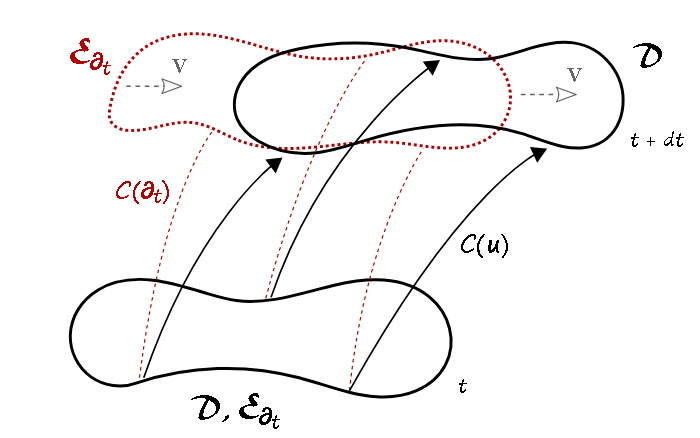
\includegraphics[scale=0.5]{domain_transportation.png}
\end{figure}

\textcolor{blue}{Aqui seguimos buchert, mas aplicamos para a congruencia de $n^\mu$}

This figure represents how the hypersurface $\Sigma$ is transported along the congruence $C(n)$, with $X^i=\text{const.}$. 
And is transported along the congruence $C(\partial_t)$, with $x^i=\text{const.}$, which coincides with $\Sigma$ at the time $t$. 
The domain undergoes a spatial motion, with velocity $\mathbf{\beta}$, in the coordinate basis $(t,x^i)$. Therefore $d/dt$ and $\int_\Sigma d^3x$ do not commute.

Consider a family of maps, $\bm{\Phi}_t=\mathbf{f}(t,\cdot)$, in order to change the coordinates $x^i$ to $X^i$,
\begin{equation}
	x^i = f^i(t,\mathbf{X}), \qquad d^3x = \text{det}\left(\frac{\partial \mathbf{f}(t,\mathbf{X})}{\partial \mathbf{X}}\right)d^3X = J(t,\mathbf{X})d^3X,
\end{equation}
while the domain transforms as, $\Sigma_x \rightarrow \Sigma_X = \mathbf{\Phi}^{-1}_t(\Sigma_x)$, the volume of the domain is then given by,
\begin{equation}
	V_\Sigma(t)=\int_{\Sigma_x}d^3x \sqrt{h(t,x^i)} \rightarrow V_\Sigma(t)=\int_{\Sigma_X}d^3X J(t,\mathbf{X})\sqrt{h(t,f^i(t,\mathbf{X}))}.
\end{equation}

The total derivative of coordinate time of the volume of domain,
\begin{align}
	\frac{d V_\Sigma}{dt} &= \int_{\Sigma_X}d^3X  \frac{d}{dt}\left(J(t,\mathbf{X})\sqrt{h(t,f^i(t,\mathbf{X}))}\right)=\int_{\Sigma_X}d^3x J^{-1} \frac{d}{dt}\left(J \sqrt{h}\right)=\\
	&=\int_{\Sigma_X}d^3x \left(\frac{d}{dt}\sqrt{h} - J \sqrt{h} \frac{d}{dt}\left(J^{-1}\right)\right)=\\
	&=\int_{\Sigma_X}d^3x \left(\partial_t\sqrt{h}-\beta^k\partial_k \sqrt{h} + J^{-1} \sqrt{h} \frac{d}{dt}J\right)
\end{align}
something useful here is,
\begin{align}
	\beta^i&=-\left.\frac{dx^i}{dt}\right|_{\mathbf{X}}=-\frac{d f^i(t,\mathbf{X})}{dt}=-\partial_t|_{\mathbf{X}} f^i(t,X) \Leftrightarrow \times \frac{d}{dX^i}\\
	\Leftrightarrow J \partial_i \beta^i &=- \partial_{X^i} \partial_t|_{\mathbf{X}} f^i(t,X) \Leftrightarrow \\
	\Leftrightarrow J \partial_i \beta^i &=- \partial_t|_{\mathbf{X}}  \partial_{X^i} f^i(t,X)\Leftrightarrow \\
	\Leftrightarrow J \partial_i \beta^i &=- \partial_t|_{\mathbf{X}}  J
\end{align}
\begin{align}
	\frac{d V_\Sigma}{dt} &=\int_{\Sigma_X}d^3x \left(\partial_t\sqrt{h}-\beta^k\partial_k \sqrt{h} - \sqrt{h} \partial_k \beta^k\right)\Leftrightarrow\\
	&=\int_{\Sigma_X}d^3x \left(\frac{1}{2}\sqrt{h} h^{ij}\partial_t h_{ij}-\frac{1}{2} h^{ij}\sqrt{h}\beta^k\partial_k h_{ij} - \sqrt{h} \partial_k \beta^k\right)=\\
	&=\int_{\Sigma_X}d^3x \sqrt{h} \left(\frac{1}{2} h^{ij}\partial_t h_{ij}-\frac{1}{2} h^{ij}\beta^k\partial_k h_{ij} - \partial_k \beta^k\right)=\\
	&=\int_{\Sigma_X}d^3x \sqrt{h} \left(\frac{1}{2} h^{ij}\partial_t h_{ij}-D_k\beta^k\right)
\end{align}
By the trace of Eq.(\ref{eqn:metric_evolution_basis}) we see that,
\begin{equation}
	\frac{d V_\Sigma}{dt} =\int_{\Sigma_X}d^3x \sqrt{h}\left(NK\right)
\end{equation}
where $D_k$ is the three-covariant derivative.
Now diving by the volume we obtain,
\begin{equation}
	\frac{1}{V_\Sigma}\frac{d V_\Sigma}{dt} = \left\langle NK \right\rangle_{\Sigma}
	\label{eqn:general_volume_buchert}
\end{equation}

The commutative relation between the time derivative and the averaging operator is given by,
\begin{equation}
	\left[\frac{d}{dt}, \langle\cdot \rangle_{\Sigma}\right] S=\left\langle NKS\right\rangle_{\Sigma}-\left\langle NK \right\rangle_{\Sigma}\langle S\rangle_{\Sigma},
	\label{eqn:comoving_commutation_rule_buchert}
\end{equation}






\section{Lightcone Averaging Procedure}

The averaging formalism made by Buchert in which we average over hypersurfaces at fixed proper times is not sufficient for observations dealing with photon detection, as photons travel along the null light-cone, a light-cone averaging procedure would be more observationally meaningful\cite{Gasperini_2011}.

In this procedure we still obtain Buchert's equations, by utilizing the Buchert-Ehlers commutation rules\cite{Gasperini_2010}. Another advantage in this procedure is that the fluid flow vector is not necessarily orthogonal to the hypersurface.

A scalar field, $S(x)$, under a 4-dimensional domain $\Omega$ in $\mathcal{M}_4$ with coordinates $x^\mu$, is given by,
\begin{equation}
    F(S,\Omega)=\int_\Omega d^4x \sqrt{-g}S(x),
\end{equation}
this expression is not generally gauge invariant, because the region $\Omega$ depends on the choice of coordinates. Gauge invariance can be achieved by introducing a window function $\mathcal{W}_\Omega(x)$ which acts as a filtering of the main manifold $\mathcal{M}_4$ to the domain in interest $\Omega$, where,
\begin{equation}
    F(S,\Omega)=\int_\Omega d^4x \sqrt{-g}S(x)\equiv \int_{\mathcal{M}_4} d^4x \sqrt{-g}S(x)\mathcal{W}_\Omega (x),
\end{equation}
where the window function will require a region, inside the past light-cone of the observer, bounded by the hypersurface of the past $A(x)=A_0$,
\begin{equation}
F(S;\underbrace{-}_{\text{Dirac}};\underbrace{A_0,V_0}_{\text{Heavyside}})=\int_{\mathcal{M}_4} d^4x \sqrt{-g}\Theta(A(x)-A_0)\Theta(V_0-V(x))S(x),
\end{equation}
where $V(x)$ is a scalar satisfying $\partial_\mu V\partial^\mu V=0$; where $V_0$ specifies the past light-cone of the observer; and where $"-"$ symbolises there are no Dirac delta functions in the window function.



\section{Conformal LCA}

In this section, we will look at how the lightcone averaging procedure changes under a conformal transformation. Immediately, the integral over a scalar function $S$, changes in the following manner,
\begin{align}
    I(S;A_0;V_0)&=\int_{\mathcal{M}}d^4x \sqrt{-g} \delta(A-A_0)\Theta(V_0-V)\sqrt{-\partial_\mu A\partial^\mu A}S(x)=\nonumber\\
    &=\int_{\mathcal{M}}d^4x \sqrt{-\Tilde{g}}\Omega^4 \delta(A-A_0)\Theta(V_0-V)\sqrt{-g^{\mu\nu}\partial_\mu A\partial_\nu A}S(x)=\nonumber\\
    &=\int_{\mathcal{M}}d^4x \sqrt{-\Tilde{g}}\Omega^3 \delta(A-A_0)\Theta(V_0-V)\sqrt{-\Tilde{g}^{\mu\nu}\partial_\mu A\partial_\nu A}S(x)=\nonumber\\
    &=\Tilde{I}(S\Omega^3;A_0;V_0)
    \label{eqn:LCA_relation_integral}
\end{align}
where we take into consideration that $A(x)$ and $V(x)$ are true scalars, and not scalars through the contraction of indices, and therefore remain unchanged, however $\sqrt{-\partial_\mu A\partial^\mu A}$ is a scalar by contraction of indices and therefore a metric tensor is present. Here we also defined the conformal integral as,
\begin{equation}
    \Tilde{I}(S;A_0;V_0) := \int_{\mathcal{M}}d^4x \sqrt{-\Tilde{g}} \delta(A-A_0)\Theta(V_0-V)\sqrt{-\Tilde{\nabla}_\mu A\Tilde{\nabla}^\mu A}S(x),
\end{equation}
where the new window function will filter the manifold into a conformal hypersurface $\Tilde{\Sigma}_{A_0}$, in the context of conformal LCA I shall omit the $A_0$ from the hypersurface, for brevity. Here the manifold remains the same, it is not changed by the conformal transformation, this is another advantage of using the window function to filter the manifold.

Defining the conformal average as,
\begin{equation}
    \langle S \rangle_{\Tilde{\Sigma}}:= \frac{\Tilde{I}(S)}{\Tilde{I}(1)},
\end{equation}
from Eq.(\ref{eqn:LCA_relation_integral}) we can obtain the following relations,
\begin{equation}
    \langle S\rangle_{\Tilde{\Sigma}}=\frac{\left\langle S\Omega^{-3}\right\rangle_{\Sigma}}{\left\langle \Omega^{-3}\right\rangle_{\Sigma}}, \qquad \langle S\rangle_{\Sigma}=\frac{\left\langle S\Omega^{3}\right\rangle_{\Tilde{\Sigma}}}{\left\langle \Omega^{3}\right\rangle_{\Tilde{\Sigma}}}.
    \label{eqn:LCA_relation_averages}
\end{equation}

Assuming $A$ is homogeneous and $V$ does not depend on the time coordinate, a convenient way to write the conformal integral is,
\begin{align}
    \Tilde{I}(S;A_0;V_0) &= \int_{\mathcal{M}}d^4x \sqrt{-\Tilde{g}} \delta(A-A_0)\Theta(V_0-V)\sqrt{-\Tilde{\nabla}_\mu A\Tilde{\nabla}^\mu A}S(x)\nonumber\\
    &= \int_{\mathcal{M}}d^3x \left(\frac{\partial t}{\partial A}dA\right) \sqrt{-\Tilde{g}} \delta(A-A_0)\Theta(V_0-V)\sqrt{-\Tilde{g}^{\mu\nu}\Tilde{\nabla}_\mu A\Tilde{\nabla}_\nu A}S(x)\nonumber\\
    &= \int_{\mathcal{M}}d^3x dA \frac{1}{\partial_0 A}\sqrt{-\Tilde{g}} \delta(A-A_0)\Theta(V_0-V)\sqrt{-\Tilde{g}^{00}\Tilde{\nabla}_0 A\Tilde{\nabla}_0 A}S(x)\nonumber\\
    &= \int_{\mathcal{M}}d^3x dA \sqrt{-\Tilde{g}} \delta(A-A_0)\Theta(V_0-V)\frac{1}{\Tilde{N}}\frac{\sqrt{\Tilde{\nabla}_0 A\Tilde{\nabla}_0 A}}{\partial_0 A}S(x)\nonumber\\
    &= \int_{\Tilde{\Sigma}_{A_0}}d^3x \sqrt{\Tilde{h}(t_0,\vec{x})}\Theta(V_0-V)S(t_0,\vec{x}),
\end{align}
where $\sqrt{-\Tilde{g}}=\Tilde{N}\sqrt{\Tilde{h}}$ and reminder that $A_0$ is the hypersurface level chosen at a time $t_0$.

Defining the conformal volume as,
\begin{equation}
    \Tilde{V}:=\int_{\Tilde{\Sigma}}d^3\sqrt{\Tilde{h}}\Theta(V_0-V),
\end{equation}
and using \cref{eqn:def_conf_transf}, allows us to see that,
\begin{equation}
    \Tilde{V}=V\langle\Omega^{-3}\rangle_\Sigma,
\end{equation}
where if we derive w.r.t $d/dt$ and divide by $\Tilde{V}$, we obtain,
\begin{equation}
    \frac{1}{\Tilde{V}}\frac{d\Tilde{V}}{dt}=\frac{1}{V}\frac{dV}{dt}+\frac{1}{\langle\Omega^{-3}\rangle_\Sigma}\frac{d}{dt}\langle\Omega^{-3}\rangle_\Sigma.
\end{equation}

The conformal volume evolution is given by,
\begin{equation}
    \frac{1}{\Tilde{V}}\frac{d\Tilde{V}}{dt}=\left\langle \Tilde{N}\Tilde{K}\right\rangle_{\Tilde{\Sigma}}
    \label{eqn:LCA_conf_volume_evo}
\end{equation}
where the term inside the averaging operators, relates to its usual form as,
\begin{equation}
    \Tilde{N}\Tilde{K}=NK-3\frac{d}{dt}\ln\Omega.
    \label{eqn:LCA__relation_general_inside_term}
\end{equation}




The commutation rule is,
\begin{equation}
    \left[\frac{d}{dt},\langle\cdot\rangle_{\Tilde{\Sigma}}\right]S=\left\langle \Tilde{N}\Tilde{K}S\right\rangle_{\Tilde{\Sigma}}-\left\langle \Tilde{N}\Tilde{K}\right\rangle_{\Tilde{\Sigma}}\langle S\rangle_{\Tilde{\Sigma}},
\end{equation}
where $NV^i=\Tilde{N}\Tilde{V}^i$ due to $v^i$ and $\beta^i$ being conformally invariant.



 \chapter{Scalar-tensor theories}

Among modified theories of gravity, scalar-tensor theories have gained more attention than others. 
The main characteristic of these theories is the introduction of an hypothetical scalar field, such fields are also present in the standard model of particle physics and unified field theories.

This scalar field can be inserted in Dirac's Large number hypothesis, where the possibility for the Gravitational "constant" $G$ to vary in time was raised.
In fact, Robert Dicke and Carl Brans, exploited this possibility with a time dependent scalar field $\phi$ \cite{Brans_1961}.

\section{Jordan-Brans-Dicke theory}

The simplest way of introducing a time-dependent gravitational constant is represented in the so-called Jordan frame by the following action:
\begin{equation}
    S_{\text{JBD}}=\int_{\mathcal{M}} d^4x\left[ \sqrt{-g}\frac{1}{2k'}\left[R\phi-\omega \frac{\phi_{,\rho}\phi^{,\rho}}{\phi}\right]+\sqrt{-g}\mathcal{L}_m\right]
    \label{eqn:BD_action_JF}
\end{equation}
where $\omega$ is the dimensionless Brans-Dicke coupling constant, $k'=8\pi$, and $\mathcal{L}_m$ is the matter Lagrangian describing ordinary matter, i.e. any form of matter different from the scalar field $\phi$. The second term is introduced in order to make the scalar field dynamical, where the factor $\phi$ in the denominator is responsible for making $\omega$ dimensionless.

In this action, matter is not directly coupled to $\phi$, in the sense that the matter Lagrangian $\mathcal{L}_m$ does not depend on $\phi$, and is minimally coupled to $\phi$. However, in the first term we see that $\phi$ is directly coupled to the metric, via the Ricci scalar. Here the metric and scalar field describe the gravitational field, contrary to other theories where the metric alone describes it, the gravitational field together with the matter will describe the dynamics. 

\subsection{Jordan frame}

The field equations of the Brans-Dicke theory:
\begin{align}
G_{\mu\nu}=k'\left\{\frac{T_{\mu\nu}^{(m)}}{\phi}+\frac{\omega}{k'\phi^2}\left[\partial_\mu \phi \partial_\nu \phi-\frac{1}{2}g_{\mu\nu}\phi_{,\lambda}\phi^{,\lambda}\right]+\frac{1}{k'\phi}\left(\nabla_\mu\nabla_\nu\phi-g_{\mu\nu}\Box\phi\right)\right\},
\label{eqn:field_eq_metric}
\end{align}
\begin{equation}
    \Box\phi=\frac{k'T^{(m)}}{2\omega+3},
    \label{eqn:field_eq_phi}
\end{equation}
where
\begin{equation}
    T_{\mu\nu}^{(m)} := \frac{-2}{\sqrt{-g}} \frac{\delta\left(\sqrt{-g} \mathcal{L}^{(m)}\right)}{\delta g^{\mu\nu}}
    \label{eqn:def_em_tensor}
\end{equation}
is the energy-momentum tensor for ordinary matter. A full derivation of the field equations is shown in \cref{app:brans}.

In \cref{eqn:field_eq_phi}, it is clear the scalar field is sourced by matter with non zero trace, i.e. $T^{(m)}\neq 0$ (this type of matter is usually called non-conformal matter for reasons that will apparent in the next section). From the relation between matter and the scalar field in the field equation of $\phi$, one would be lead to believe there is a coupling between the two, however even in the derivation this relation only happens via the field equation of the metric, hence a minimal coupling between matter and $\phi$.

By defining an effective energy-momentum tensor as
\begin{equation}
    T^{\mathrm{eff}}_{\mu\nu}=\frac{T_{\mu\nu}^{(m)}}{\phi}+\frac{\omega}{k'\phi^2}\left[\partial_\mu \phi \partial_\nu \phi-\frac{1}{2}g_{\mu\nu}\phi_{,\lambda}\phi^{,\lambda}\right]+\frac{1}{k'\phi}\left(\nabla_\mu\nabla_\nu\phi-g_{\mu\nu}\Box\phi\right),
\end{equation}
we see that its components w.r.t the observer's four-velocity $n_\mu$, are as follows. The energy density:
\begin{align}
    E &= T_{\mu\nu}n^\mu n^\nu=\left[\frac{T^{(M)}_{\mu \nu}}{\phi}+\frac{1}{k'}\left(\frac{1}{\phi}\left(\nabla_\mu \nabla_\nu \phi-g_{\mu \nu} \square \phi\right)+\frac{\omega}{\phi^2}\left[\partial_\mu \phi \partial_\nu \phi-\frac{1}{2} g_{\mu \nu}(\nabla \phi)^2\right]\right)\right]n^\mu n^\nu\nonumber\\
    &=\frac{E_m}{\phi}+\frac{\omega}{k'\phi^2}\left((n^\mu\partial_\mu \phi)(n^\nu\partial_\nu\phi)-\frac{1}{2}g_{\mu\nu}n^\mu n^\nu (\nabla \phi)^2\right)+\frac{1}{k'\phi}\left(n^\mu n^\nu \nabla_\mu \nabla_\nu - g_{\mu\nu}n^\mu n^\nu \Box\right)\phi\nonumber\\
    &=\frac{E_m}{\phi}+\frac{\omega}{k'\phi^2}\left(\left(\frac{1}{N}\frac{d\phi}{dt}\right)^2+\frac{1}{2}(\nabla\phi)^2\right)+\frac{1}{k'\phi}\left[\frac{1}{N}\frac{d}{dt}\left(\frac{1}{N}\frac{d\phi}{dt}\right)-A^\mu\nabla_\mu\phi+\Box\phi\right]=\nonumber\\
    &=\frac{E_m}{\phi}+\frac{\omega}{k'\phi^2}\left(\frac{1}{2}\left(\frac{1}{N}\frac{d\phi}{dt}\right)^2+\frac{1}{2}h^{\mu\nu}D_\mu\phi D_\nu\phi\right)+\frac{1}{k'\phi}\left[D^\alpha D_\alpha\phi-\frac{K}{N}\frac{d\phi}{dt}\right]
    \label{eqn:energy_density_jf}
\end{align}
where we use the \cref{eqn:relation_total_time_normal_vec}. And the pressure is given by
\begin{align}
    S&=T_{\mu\nu}h^{\mu\nu}=\frac{S_m}{\phi}+\frac{\omega}{k'\phi^2}\left(\frac{3}{2}\left(\frac{1}{N}\frac{d\phi}{dt}\right)^2 -\frac{1}{2}h^{\alpha\beta} D_\alpha\phi D_\beta\phi\right)+\label{eqn:pressure_jf}\\
    &\qquad\qquad\qquad\qquad\qquad+\frac{1}{k'\phi}\left[3N\frac{d^2\phi}{dt^2}-3\frac{d\phi}{dt}\frac{dN}{dt}-3A^\mu\nabla_\mu\phi -2D^\alpha D_\alpha \phi+2\frac{K}{N}\frac{d\phi}{dt} \right],\nonumber
\end{align}
where we use $D_\mu \phi = h_\mu^\alpha \nabla_\alpha\phi \Leftrightarrow h^\mu_\beta D_\mu \phi = h^\alpha_\beta \nabla_\alpha \phi$.




It is useful to determine
\begin{align}
    E+S&=\frac{E_m+S_m}{\phi}+\frac{\omega}{k'\phi^2}\left(\frac{1}{N}\frac{d\ln\phi}{dt}\right)^2+\frac{1}{k'\phi}\left[\frac{3}{N}\frac{d}{dt}\left(\frac{1}{N}\frac{d\phi}{dt}\right)-3A^\mu\nabla_\mu\phi-D^\alpha D_\alpha\phi+\frac{K}{N}\frac{d\phi}{dt}\right].
    \label{eqn:raych_useful}
\end{align}



\subsection{Einstein frame}

In 1961, Brans and Dicke showed that under a conformal transformation, in \cref{eqn:def_conf_transf}, the Brans-Dicke action can recover a form similar to the Hilbert-Einstein action \cite{Brans_1961}, we call this the Einstein frame. This is a very common technique used in gravitational theories and cosmology, to go from the Jordan frame to the Einstein frame.


By reviewing the action in \cref{eqn:BD_action_JF}, and (eq do ricci):
\begin{align}
    S_{\text{JBD}}=&\int_{\mathcal{M}} d^4x\sqrt{-\Tilde{g}}\Omega^4\frac{1}{2k'}\left[\Omega^{-2}\left(\Tilde{R}-6\Tilde{\nabla}_\mu\Tilde{\nabla}^\mu\ln\Omega-6\Tilde{\nabla}_\mu\ln\Omega\Tilde{\nabla}^\mu\ln\Omega\right)\phi-\omega \frac{\Omega^{-2}\Tilde{\nabla}_\mu\phi\Tilde{\nabla}^\mu\phi}{\phi}\right]\nonumber\\
    &+\int_{\mathcal{M}} d^4x\sqrt{-\Tilde{g}}\Omega^4\mathcal{L}_m(\Omega^{-2}\Tilde{g}^{\mu\nu},\Psi),
    \label{eqn:bd_ef_1}
\end{align}
where if we choose the conformal factor to be
\begin{equation}
    \Omega^2=(G\phi)^{-1},
\end{equation}
the corresponding action will be
\begin{align}
    S_{\text{EF}}=&\int_{\mathcal{M}} d^4x\sqrt{-\Tilde{g}}\frac{1}{2k}\left[\Tilde{R}+3\Tilde{\nabla}_\mu\Tilde{\nabla}^\mu\ln\phi-\frac{3}{2}\Tilde{\nabla}_\mu\ln\phi\Tilde{\nabla}^\mu\ln\phi-\omega \frac{\Tilde{\nabla}_\mu\phi\Tilde{\nabla}^\mu\phi}{\phi^2}\right]\nonumber\\
    &+\int_{\mathcal{M}} d^4x\sqrt{-\Tilde{g}}\Omega^4\mathcal{L}_m(\Omega^{-2}\Tilde{g}^{\mu\nu},\Psi),
    \label{eqn:bd_ef_2}
\end{align}
and hence, we obtain an action written in the Einstein frame. We can further simplify by noting the second term, inside the square brackets, is a surface term and therefore is removed from our action, turning our action into:
\begin{align}
    S_{\text{EF}}=&\int_{\mathcal{M}} d^4x\sqrt{-\Tilde{g}}\left[\frac{\Tilde{R}}{2k}-\frac{1}{2k}\left(\frac{3}{2}+\omega\right)\Tilde{\nabla}_\mu\ln\phi\Tilde{\nabla}^\mu\ln\phi+\Omega^4\mathcal{L}_m(\Omega^{-2}\Tilde{g}^{\mu\nu},\Psi)\right].
    \label{eqn:bd_ef_3}
\end{align}

We can define a new scalar field $\varphi$ as
\begin{equation}
    \varphi =\sqrt{\frac{3+2\omega}{2k}}\ln\phi.
\end{equation}

In \cref{eqn:bd_ef_3}, we still do not have the matter Lagrangian written in the Einstein frame. In fact, depending on the ordinary matter being treated, this will acquire vastly different situations. These differences are due to two types of matter: 

\textbf{Conformal matter}, the Lagrangian scales with the conformal factor in the following way:
\begin{equation}
\mathcal{L}_m(g^{\mu\nu}\Omega^{-2},\Psi)=\Omega^{-4}\mathcal{L}_m(\Tilde{g}^{\mu\nu},\Psi),
\end{equation}
therefore making $\sqrt{-g}\mathcal{L}_m$ conformally invariant. This scaling can arise, for example, in radiation fields and scalar fields with a zero or quadratic potential. For example, the Maxwell field:
\begin{align}
     \mathcal{L}_m(g^{\mu\nu},A_\mu)&=-\frac{1}{4}F^{\mu\nu}F_{\mu\nu}=-\frac{1}{4}g^{\mu\alpha}g^{\nu\beta}F_{\alpha\beta}F_{\mu\nu}=-\frac{1}{4}\Omega^{-4}\Tilde{g}^{\mu\alpha}\Tilde{g}^{\nu\beta}F_{\alpha\beta}F_{\mu\nu}=\nonumber\\
     &=\Omega^{-4}\mathcal{L}_m(\Tilde{g}^{\mu\nu},\Tilde{A}_\mu),
\end{align}
where the Maxwell tensor is and has $\Tilde{F}_{\alpha\beta}=F_{\alpha\beta}$.

From \cref{eqn:def_em_tensor}, the energy-momentum tensor scales by
\begin{equation}
    T_{\mu\nu}=\Omega^2\Tilde{T}_{\mu\nu},
\end{equation}
and is traceless, i.e. $T=T^\mu_\mu=0$. This choice is seen in Brans' paper of 1961 \cite{Brans_1961}, and this recent paper \cite{quiros2025}, contains proofs for a radiative field, a fermionic field and a perfect fluid.

\textbf{Non-conformal matter}, where the Lagrangian does not scale with the conformal factor, and therefore, from \cref{eqn:def_em_tensor}, the energy-momentum tensor scales as
\begin{equation}
    T_{\mu\nu}=\Omega^{-2}\Tilde{T}_{\mu\nu},
\end{equation}
and has a non zero trace. With this matter we obtain a coupling between the matter Lagrangian and the conformal factor.

\textcolor{blue}{Deixar claro qual o tipo de materia que se vai usar}

Therefore, the action in \cref{eqn:bd_ef_3}:
\begin{equation}
    S_{\text{EF}}=\int_{\mathcal{M}} d^4x\sqrt{-\Tilde{g}}\left[\frac{\Tilde{R}}{2k}-\frac{1}{2}\Tilde{\nabla}_\mu\varphi\Tilde{\nabla}^\mu\varphi+\frac{1}{G^2\phi^2}\mathcal{L}_m(\Tilde{g}^{\mu\nu},\Psi)\right].
    \label{eqn:bd_ef_4}
\end{equation}

With help from the \cref{app:brans}, we can determine the variation w.r.t the metric of the Einstein frame's action to be
\begin{equation}
    \delta_{\Tilde{g}} S = \int_{\mathcal{M}} d^4x\sqrt{-\Tilde{g}} \delta \Tilde{g}^{\mu\nu}\left\{\frac{\Tilde{G}_{\mu\nu}}{2k}-\frac{1}{2}\left(\Tilde{\nabla}_\mu\varphi\Tilde{\nabla}_\nu\varphi-\frac{1}{2}g_{\mu\nu}\Tilde{\nabla}_\lambda\varphi\Tilde{\nabla}^\lambda\varphi\right)-\frac{1}{2}\alpha(\varphi)\Tilde{T}_{\mu\nu}^{(m)}\right\}
\end{equation}
where $\alpha(\varphi)=\exp\left(-2\sqrt{\frac{2k}{3+2\omega}}\varphi\right)/G^2$ refers to the coupling between matter and the field $\varphi$. And w.r.t the scalar field:
\begin{equation}
    \delta_\varphi S=  \int_{\mathcal{M}} d^4x\sqrt{-\Tilde{g}}\delta\varphi \Tilde{\Box}\varphi +\delta_\varphi S_m(g^{\mu\nu}).
\end{equation}
The extra term can be varied as
\begin{equation}
    \delta_\varphi S_m(g^{\mu\nu})=\delta_{\varphi} g^{\mu\nu} \frac{\delta S_m(g^{\mu\nu})}{\delta g^{\mu\nu}}=-\frac{1}{2}\sqrt{\frac{2\kappa^2}{2\omega+3}}(-\rho_m+3P_m).
\end{equation}

By taking $\delta_{\Tilde{g}} S=0$ and $\delta_\varphi S=0$, we obtain the following field equations:
\begin{align}
    &\Tilde{G}_{\mu\nu}=k\left\{ \alpha(\varphi)\Tilde{T}_{\mu\nu}^{(m)} + \left(\Tilde{\nabla}_\mu\varphi\Tilde{\nabla}_\nu\varphi-\frac{1}{2}g_{\mu\nu}\Tilde{\nabla}_\lambda\varphi\Tilde{\nabla}^\lambda\varphi\right) \right\},\label{eqn:field_metric_ef}\\
    &\Tilde{\Box}\varphi=\frac{1}{2}\sqrt{\frac{2\kappa^2}{2\omega+3}}(-\rho_m+3P_m).\label{eqn:field_scalar_ef}
\end{align}


As seen in the Jordan frame, we can write the RHS of \cref{eqn:field_metric_ef}, as an effective energy-momentum tensor (conformal) given by
\begin{equation}
    \Tilde{T}^{\mathrm{eff}}_{\mu\nu}:=\alpha(\varphi)\Tilde{T}_{\mu\nu}^{(m)} + \Tilde{\nabla}_\mu\varphi\Tilde{\nabla}_\nu\varphi-\frac{1}{2}g_{\mu\nu}\Tilde{\nabla}_\lambda\varphi\Tilde{\nabla}^\lambda\varphi,
\end{equation}
and its energy density according to the conformal observer is
\begin{equation}
    \Tilde{E}=\Tilde{T}^{\mathrm{eff}}_{\mu\nu}\Tilde{n}^\mu\Tilde{n}^\nu =\alpha(\varphi)\Tilde{E}_m+\frac{1}{2}\left(\frac{1}{\Tilde{N}}\frac{d\varphi}{dt}\right)^2+\frac{1}{2}\Tilde{D}_\lambda\varphi\Tilde{D}^\lambda\varphi,
    \label{eqn:energy_density_ef}
\end{equation}
and the pressure is
\begin{equation}
\Tilde{S}=\Tilde{T}^{\mathrm{eff}}_{\mu\nu}\Tilde{h}^{\mu\nu}=3\alpha(\varphi)\Tilde{S}_m+\frac{3}{2}\left(\frac{1}{\Tilde{N}}\frac{d\varphi}{dt}\right)^2-\frac{1}{2}\Tilde{D}_\lambda\varphi\Tilde{D}^\lambda\varphi
    \label{eqn:pressure_ef}
\end{equation}



In this frame, due to the direct coupling between matter and the scalar field, the conservation law of the matter EM tensor transforms as
\begin{align}
    \tilde{\nabla}_\alpha\tilde{T}^{\alpha\beta}_{(m)}&=\tilde{\nabla}_\alpha\left(\Omega^{6} T_{(m)}^{\alpha\beta}\right)=\nabla_\alpha\left(\Omega^{6} T_{(m)}^{\alpha\beta}\right)+\Omega^6\left(C^\alpha_{\alpha\lambda}T_{(m)}^{\lambda\beta}+C^\beta_{\alpha\lambda}T_{(m)}^{\alpha\lambda}\right)\nonumber\\
    &=\Omega^6 \nabla_\alpha T_{(m)}^{\alpha\beta}+6 \Omega^{5} T_{(m)}^{\alpha\beta} \nabla_\alpha \Omega-\Omega^5\left[4T_{(m)}^{\lambda\beta} \nabla_\lambda \Omega + T_{(m)}^{\alpha\lambda}\left(\delta^\beta_\alpha\nabla_\lambda + \delta^\beta_\lambda \nabla_\alpha- \tilde{g}_{\alpha\lambda}\nabla^\beta\right)\Omega\right] \nonumber\\
    &=\Omega^6 \nabla_\alpha T_{(m)}^{\alpha\beta}+6 \Omega^{5} T_{(m)}^{\alpha\beta} \nabla_\alpha \Omega-\Omega^5\left[4T_{(m)}^{\lambda\beta} \nabla_\lambda \Omega +\left( T_{(m)}^{\beta\lambda}\nabla_\lambda +  T_{(m)}^{\alpha\beta}\nabla_\alpha-  T_{(m)}\Omega^{-2}\nabla^\beta\right)\Omega\right]\nonumber\\
    &=\Omega^6 \nabla_\alpha T_{(m)}^{\alpha\beta}+\Omega^3 T^{(m)}\nabla^\beta\Omega=\Omega^3 T^{(m)}\nabla^\beta\Omega.
    \label{eqn:conserv_law_conf_1}
\end{align}


By noticing the trace of the EM tensor transforms as
\begin{equation}
    \tilde{T}^{(m)} \equiv \tilde{g}^{\alpha\beta} \tilde{T}_{\alpha\beta}^{(m)}=\Omega^{4} T^{(m)} .
\end{equation}

Therefore, $\tilde{T}^{(m)}$ vanishes iff. $T^{(m)}=0$. Then \cref{eqn:conserv_law_conf_1} becomes
\begin{equation}
    \tilde{\nabla}_\alpha \tilde{T}_{(m)}^{\alpha\beta}=\tilde{T}^{(m)}\tilde{\nabla}^\beta(\ln \Omega).
\end{equation}


In the JBD theory the choice of transfomation is $\Omega=(G \phi)^{-1/2}$, then we obtain
\begin{equation}
    \tilde{\nabla}_\alpha \tilde{T}_{(m)}^{\alpha\beta}=-\frac{1}{2} \tilde{T}^{(m)} \tilde{\nabla}^\beta \ln\phi,
\end{equation}


or, in terms of the new scalar field:
\begin{equation}
    \tilde{\nabla}_\alpha \tilde{T}_{(m)}^{\alpha\beta}=-\frac{1}{2}\sqrt{\frac{2\kappa^2}{2\omega+3}} \tilde{T}^{(m)} \tilde{\nabla}^\beta \varphi.
\end{equation}


\section{Bergmann-Wagoner theory}

Bergmann \cite{Bergmann1968} and Wagoner \cite{wagoner1970} proposed the most general scalar-tensor theory of gravitation, by introducing a cosmological function $\Lambda(\phi)$ and a $\phi$-dependent coupling, $\omega:=\omega(\phi)$, yield the following action:
\begin{equation}
    S_{\text{BW}}=\int_{\mathcal{M}} d^4x\left[ \sqrt{-g}\frac{1}{2k'}\left[R\phi-\omega \frac{\phi_{,\rho}\phi^{,\rho}}{\phi}-V(\phi)\right]+\sqrt{-g}\mathcal{L}_m\right].
    \label{eqn:BD_action_JF}
\end{equation}

It can be shown that the JBD theory is a special case of BW theory, by
\begin{equation}
    \omega(\phi)=\omega=C^{te},\qquad \Lambda(\phi)=0.
\end{equation}

Under the variational principle, the variation w.r.t the metric, will be the same as in \cref{eqn:appendix_delta_metric} with an extra term:
\begin{equation}
    \delta_g \int_{\mathcal{M}}d^4x\sqrt{-g}\frac{1}{2k'}\Lambda(\phi) = \frac{1}{2k'}\int_{\mathcal{M}}d^4x\sqrt{-g}\left(\frac{1}{2}\Lambda(\phi)g_{\mu\nu}\right),
\end{equation}
this will yield the following field equation:
\begin{align}
G_{\mu\nu}=k'\left\{\frac{T_{\mu\nu}^{(m)}}{\phi}+\frac{\omega}{k'\phi^2}\left[\partial_\mu \phi \partial_\nu \phi-\frac{1}{2}g_{\mu\nu}\phi_{,\lambda}\phi^{,\lambda}\right]+\frac{1}{k'\phi}\left(\nabla_\mu\nabla_\nu\phi-g_{\mu\nu}\Box\phi\right)-\frac{\Lambda(\phi)g_{\mu\nu}}{2k'\phi}\right\}.
\label{eqn:field_eq_metric_bw}
\end{align}

The variation w.r.t the scalar field, will be
\begin{equation}
    \delta_\phi S_{\mathrm{BW}}=\frac{1}{2k'}\int_{\mathcal{M}} d^4x\sqrt{-g}\left\{ R-\left(\frac{\omega}{\phi}+\frac{d\omega(\phi)}{d\phi}\right)\frac{\phi_{,\mu}\phi^{,\mu}}{\phi}+2\omega\frac{\Box\phi}{\phi}-\frac{d\Lambda(\phi)}{d\phi}\right\}\delta\phi
    \label{eqn:delta_phi_bw}
\end{equation}
which with $\delta_\phi S_{\mathrm{BW}}=0$ and the trace of \cref{eqn:field_eq_metric_bw}:
\begin{align}
    2\omega\Box\phi&=-\phi R+\left(\frac{\omega}{\phi}+\frac{d\omega(\phi)}{d\phi}\right)\phi_{,\mu}\phi^{,\mu}+\phi\frac{d\Lambda(\phi)}{d\phi}\Leftrightarrow\nonumber\\
    \Leftrightarrow 2\omega\Box\phi&=\phi\left[\frac{k'T^{(m)}}{\phi}-\omega\frac{\phi_{,\mu}\phi^{,\mu}}{\phi^2}-3\frac{\Box\phi}{\phi}\right]+\left(\frac{\omega}{\phi}+\frac{d\omega(\phi)}{d\phi}\right)\phi_{,\mu}\phi^{,\mu}+\phi\frac{d\Lambda(\phi)}{d\phi}\Leftrightarrow\nonumber\\
    \Leftrightarrow (2\omega+3)\Box\phi &=k' T^{(m)}+\frac{d\omega(\phi)}{d\phi}\phi_{,\mu}\phi^{,\mu}+\phi\frac{d\Lambda(\phi)}{d\phi}
\end{align}


\subsection{Einstien frame}

\begin{equation}
    S_{\text{EF}}=\int_{\mathcal{M}}d^4x \sqrt{-\tilde{g}}\left[\frac{\tilde{R}}{2k}-\frac{1}{2k}\left(\frac{3}{2}+\omega\right)\tilde{g}^{\mu\nu}\phi_{,\mu}\phi_{,\nu}-\frac{1}{2k}\frac{\Lambda(\phi)}{G\phi^2}+\alpha(\phi)\mathcal{L}_m(\tilde{g}^{\mu\nu},\Psi)\right]
\end{equation}



\chapter{Backreaction}


\section{Jordan-Brans-Dicke theory}

\subsection{Jordan frame}

The scale factor is given by,
\begin{equation}
    \frac{a_\Sigma}{a_{\Sigma_0}}:=\left(\frac{V_\Sigma}{V_{\Sigma_0}}\right)^{1/3}.
\end{equation}

The effective Hubble expansion is thus defined as,
\begin{equation}
    H_{\Sigma} := \frac{1}{a_{\Sigma}}\frac{da_{\Sigma}}{dt}\equiv \frac{1}{3V_{\Sigma}}\frac{dV_{\Sigma}}{dt}\equiv\frac{1}{3}\left\langle NK \right\rangle_{\Sigma}.
    \label{eqn:def_scale_factor}
\end{equation}

\begin{align}
    \frac{1}{a}\frac{d^2a}{dt^2}&=\frac{d}{dt}\left(\frac{1}{a}\frac{da}{dt}\right)+\left(\frac{1}{a}\frac{da}{dt}\right)^2=\frac{1}{3}\frac{d}{dt}\left\langle NK \right\rangle_{\Sigma}+\frac{1}{9}\left\langle NK \right\rangle_{\Sigma}^2\nonumber\\
    &=\frac{1}{3}\left\langle \frac{d}{dt}(NK) \right\rangle_{\Sigma}+\frac{1}{3}\langle N^2K^2\rangle_{\Sigma}-\frac{1}{3}\langle NK\rangle^2_\Sigma+\frac{1}{9}\left\langle NK \right\rangle_{\Sigma}^2\nonumber\\
    &=\frac{1}{3}\left\langle \frac{d}{dt}(NK) \right\rangle_{\Sigma}+\frac{1}{3}\langle N^2K^2\rangle_{\Sigma}-\frac{2}{9}\langle NK\rangle^2_\Sigma
    \label{eqn:useful_51}
\end{align}


The objective now is to obtain a Friedmannian equation, we can do this by taking the energy equation in \cref{eqn:energy_equation}, multiplying by $N^2$ and taking the average,
\begin{equation}
    k\langle N^2E\rangle=\frac{1}{2}\langle N^2\prescript{3}{}{R}\rangle+\frac{1}{2}\langle N^2(K^2+K_{ij}K^{ij})\rangle,
\end{equation}
from here by summing $3\left(\frac{1}{a}\frac{da}{dt}\right)^2$ on the RHS and $\frac{1}{3}\langle NK\rangle^2$ on the LHS, as they are the same, the equation still stands, and after rearranging we get the following equation,
\begin{equation}
    3\left(\frac{1}{a}\frac{da}{dt}\right)^2=k\langle N^2E\rangle-\frac{1}{2}\langle N^2\prescript{3}{}{R}\rangle-\frac{1}{2}\left[\left\langle N^2(K^2+K_{ij}K^{ij})\right\rangle-\frac{2}{3}\langle NK\rangle^2\right].
\end{equation}


Now for the Raychaudhuri equation, by summing the \cref{eqn:energy_equation,eqn:pressure_equation}, multiplying by $N^2$ and taking the average,
\begin{equation}
    \frac{k}{2}\langle N^2(E+S)\rangle_\Sigma=-\left\langle N\frac{dK}{dt}\right\rangle_\Sigma+\langle N^2K_{ij}K^{ij}\rangle_\Sigma+\langle ND_iD^iN\rangle_\Sigma,
\end{equation}
from here by summing $3\frac{1}{a}\frac{d^2a}{dt^2}$ on the LHS and the expression of \cref{eqn:useful_51} on the RHS, we obtain,
\begin{equation}
    3\frac{1}{a}\frac{d^2a}{dt^2}=-\frac{k}{2}\langle N^2(E+S)\rangle_\Sigma+\left\langle N^2(K^2+K_{ij}K^{ij})\right\rangle_{\Sigma}-\frac{2}{3}\langle NK\rangle^2_\Sigma+\left\langle ND_iD^i N+K\frac{dN}{dt}\right\rangle.\nonumber
\end{equation}





The averaged Friedman and Raychaudhuri equations as,
\begin{align}
    &3\left(\frac{1}{a_\Sigma}\frac{da_\Sigma}{dt}\right)^2=k'E_{\mathrm{eff}},\label{eqn:friedman_eqs_jf_1}\\
    &3\frac{1}{a_{\Sigma}}\frac{d^2a_{\Sigma}}{dt^2}=-\frac{k'}{2}\left(E_{\mathrm{eff}}+S_{\mathrm{eff}}\right)\label{eqn:raychaud_eqs_jf_1}
\end{align}
where $E_{\mathrm{eff}}$ and $S_{\mathrm{eff}}$ are the effective energy density and pressure according to the observer,
\begin{align}
    &E_{\mathrm{eff}}:=\left\langle N^2E\right\rangle_{\Sigma}-\frac{1}{2k'}\left(\mathcal{R}_\Sigma+\mathcal{Q}_{\Sigma}\right),
    \label{eqn:E_eff_1}\\
    &S_{\mathrm{eff}}:=\left\langle N^2 S\right\rangle_{\Sigma}-\frac{1}{2k'}\left[3\mathcal{Q}_{\Sigma}+4\mathcal{P}_{\Sigma}-\mathcal{R}_\Sigma\right]\label{eqn:S_eff_1}
\end{align}
where the kinematical and dynamical backreactions are defined as \cite{Buchert_2020}, 
\begin{align}
    \mathcal{R}_\Sigma :=&\left\langle N^2 \prescript{(3)}{}{R}\right\rangle_{\Sigma}\\
    \mathcal{Q}_{\Sigma}:=& \left\langle N^2\left(K^2+K_{ij}K^{ij}\right)\right\rangle_{\Sigma}-\frac{2}{3}\left\langle NK\right\rangle_{\Sigma}^2, \\
    \mathcal{P}_{\Sigma}:= &\left\langle N D_i D^i N+K\frac{dN}{dt}\right\rangle_{\Sigma},
\end{align}

\textcolor{blue}{verificar invariancia de gauge}







By expressing the effective energy density and pressure in \cref{eqn:E_eff_1,eqn:S_eff_1}, with \cref{eqn:energy_density_jf,eqn:pressure_jf},
\begin{align}
    &E_{\mathrm{eff}} = \left\langle N^2 \rho\right\rangle_{\Sigma}-\frac{1}{2k'}\left(\mathcal{R}_\Sigma+\mathcal{Q}_{\Sigma}+\sum_a \mathcal{T}^{(a)}_{\Sigma}\right),\\
    &S_{\mathrm{eff}}:=3\left\langle N^2 P\right\rangle_{\Sigma}-\frac{1}{2k'}\left[3\mathcal{Q}_{\Sigma}+4\mathcal{P}_{\Sigma}-\mathcal{R}_\Sigma+\sum_a\mathcal{T}^{(a)}_{\Sigma}\right],
\end{align}
where we introduce a new kind of backreaction, the stress energy backreaction $\mathcal{T}^{(a)}_\Sigma$, in which the index $a$ refers to the species (matter, radiation or scalar field), in order to express the matter energy density and pressure according to the fluid flow, $\rho_m$ and $P_m$, where it is given by,
\begin{equation}
    \mathcal{T}^{(a)}_{\Sigma}=-2k\left\langle N^2\left(n^\mu n^\nu-u^\mu_{(a)} u^\nu_{(a)}\right)T_{\mu\nu}^{(a)}\right\rangle_\Sigma,
\end{equation}
where $u_{(a)}^\mu$ is the four-velocity of the corresponding species $(a)$.



\textcolor{blue}{Como diferenciar termos cinematicos de termos dinamicos}




A necessary condition for \cref{eqn:friedman_eqs_jf_1} to yield \cref{eqn:raychaud_eqs_jf_1} is the integrability condition given by \cite{Buchert_2020},
\begin{align}
\begin{gathered}
\frac{1}{a_\Sigma^6}\left[\frac{d}{d t}\left(a_\Sigma^6\mathcal{Q}_{\Sigma}\right)+a_\Sigma^4\frac{d}{dt}\left(a_\Sigma^2\mathcal{R}_{\Sigma}\right)+a_\Sigma^2\frac{d}{dt}\left(a_\Sigma^4 \mathcal{T}_{\Sigma}\right)+4a_\Sigma^5\frac{da_\Sigma}{dt}\mathcal{P}_{\Sigma}\right]=\nonumber \\
=2k\left(\frac{d}{d t}\left\langle N^2 \rho\right\rangle_{\Sigma}+\frac{3}{a_{\Sigma}} \frac{d a_{\Sigma}}{d t}\left\langle N^2(\rho+P)\right\rangle_{\Sigma}\right),
\end{gathered}
\end{align}
where the LHS are the various backreactions and in the RHS is an "averaged" continuity equation. To prove this, take the continuity equation in (cref), by multiplying $\times N^3$ and taking its average we get,
\begin{align}
    \left\langle N^2\frac{d E}{dt}\right\rangle + \left\langle N\Theta N^2(E+S)\right\rangle =  -\left\langle N^3\left( 2 A_\alpha J^\alpha +  D_\alpha J^\alpha+ S^{\alpha\beta}A_{\alpha\beta}\right)\right\rangle,
\end{align}
where via the commutation rule in \cref{eqn:comoving_commutation_rule_buchert}, the relation in , and the scale factor in \cref{eqn:def_scale_factor}, we obtain,
\begin{align}
    &\frac{d}{dt}\left\langle N^2\rho\right\rangle+3\frac{1}{a_\Sigma}\frac{da_\Sigma}{dt}\langle N^2(\rho+P)\rangle=3\frac{1}{a_\Sigma}\frac{da_\Sigma}{dt}\langle N^2P\rangle+\left\langle \left(2\frac{d\ln N}{dt}-\frac{d\ln \Gamma}{dt}\right)N^2\rho\right\rangle\\
    &-\left\langle\left(NK+\frac{d\ln\Gamma}{dt}\right)N^2P\right\rangle-\left\langle \frac{N^3}{\Gamma}\left(2A_\alpha q^\alpha+D^{(u)}_\alpha q^\alpha\right)\right\rangle
\end{align}
\textcolor{red}{corrigir para n}



\subsection{Homogeneous scalar field}

Let us consider a homogeneous field $\phi=\phi(t)$, in this scenario we have,
\begin{align}
    &(\nabla\phi)^2=g^{00}(\partial_0\phi)^2=-\frac{1}{N^2}\left(\frac{d\phi}{dt}\right)^2, \qquad A^\mu\nabla_\mu\phi=g^{0i}A_i\nabla_0\phi=-\frac{\beta^i A_i}{N^2}\frac{d\phi}{dt}\\
    &\Box\phi=g^{00}\nabla_0\nabla_0\phi=-\frac{1}{N^2}\frac{d^2\phi}{dt^2},\qquad \frac{1}{N}\frac{d}{dt}\left(\frac{1}{N}\frac{d\phi}{dt}\right)=\frac{1}{N^2}\left[\frac{d\phi}{dt}\frac{d}{dt}\ln\left(\frac{1}{N}\right)+\frac{d^2\phi}{dt^2}\right]
\end{align}










\subsection{Einstein frame}

The effective conformal scale factor is given by,
\begin{equation}
    \frac{\Tilde{a}_{\Tilde{\Sigma}}}{\Tilde{a}_{\Tilde{\Sigma}_0}}:=\left(\frac{\Tilde{V}_{\Tilde{\Sigma}}}{\Tilde{V}_{\Tilde{\Sigma}_0}}\right)^{1/3}.
\end{equation}

The effective conformal Hubble expansion is thus defined as,
\begin{equation}
    \Tilde{H} := \frac{1}{\Tilde{a}}\frac{d\Tilde{a}}{dt}\equiv \frac{1}{3\Tilde{V}}\frac{d\Tilde{V}}{dt}\equiv\frac{1}{3}\left\langle \Tilde{N}\Tilde{K} \right\rangle_{\Tilde{\Sigma}}.
\end{equation}

From the same procedure as in the Jordan frame, the averaged conformal Friedman equation are,
\begin{align}
    &3\left(\frac{1}{\Tilde{a}}\frac{d\Tilde{a}}{dt}\right)^2 = k\left\langle \Tilde{N}^2\Tilde{E}\right\rangle_{\Tilde{\Sigma}}-\frac{1}{2}\Tilde{\mathcal{R}}_{\Tilde{\Sigma}}-\frac{1}{2}\Tilde{\mathcal{Q}}_{\Tilde{\Sigma}},\\
    &3\frac{1}{\Tilde{a}_{\Tilde{\Sigma}}}\frac{d^2\Tilde{a}_{\Tilde{\Sigma}}}{dt^2}=-\frac{k}{2}\left\langle \Tilde{N}^2\left(\Tilde{E}+\Tilde{S}\right)\right\rangle_{\Tilde{\Sigma}}+\Tilde{\mathcal{Q}}_{\Tilde{\Sigma}}+\Tilde{\mathcal{P}}_{\Tilde{\Sigma}},
\end{align}
where the average intrinsic curvature, the kinematical and dynamical backreactions are defined as,
\begin{align}
    \tilde{\mathcal{Q}}_{\tilde{\Sigma}}:=& \left\langle \tilde{N}^2\left(\tilde{K}^2+\tilde{K}_{ij}\tilde{K}^{ij}\right)\right\rangle_{\tilde{\Sigma}}-\frac{2}{3}\left\langle \tilde{N}\tilde{K}\right\rangle_{\tilde{\Sigma}}^2, \\
    \tilde{\mathcal{P}}_{\tilde{\Sigma}}:=&\left\langle \tilde{N} \tilde{D}_i \tilde{D}^i \tilde{N}+\tilde{K}\frac{d\tilde{N}}{dt}\right\rangle_{\tilde{\Sigma}}.
\end{align}
and they relate to the usual backreactions by,
\begin{align}
    &\mathcal{Q}_\Sigma = \tilde{\mathcal{Q}}_{\tilde{\Sigma}} - 4 \frac{d}{dt}\ln\Omega\left\langle  \tilde{N}\tilde{K}\right\rangle_{\tilde{\Sigma}}+6\left(\frac{d}{dt}\ln\Omega\right)^2\\
    &\mathcal{P}_\Sigma = \tilde{\mathcal{P}}_{\tilde{\Sigma}}+\frac{d}{dt}\ln\Omega\left\langle \tilde{N}\tilde{K}+3\frac{d}{dt}\ln\tilde{N}\right\rangle_{\tilde{\Sigma}}+3\left(\frac{d}{dt}\ln\Omega\right)^2
\end{align}
where we assume the conformal factor to be homogeneous.

Like before, the Friedmann equations can be simplified into a more familiar form,
\begin{align}
    &3\left(\frac{1}{\Tilde{a}}\frac{d\Tilde{a}}{dt}\right)^2 = k\tilde{E}_{\mathrm{eff}},\\
    &3\frac{1}{\Tilde{a}_{\Tilde{\Sigma}}}\frac{d^2\Tilde{a}_{\Tilde{\Sigma}}}{dt^2}=-\frac{k}{2}(\tilde{E}_{\mathrm{eff}}+\tilde{S}_{\mathrm{eff}}),
\end{align}
where the effective energy density and pressure are given by the same form as in \cref{eqn:E_eff_1,eqn:S_eff_1}, and by introducing the \cref{eqn:energy_density_ef,eqn:pressure_ef}, we obtain,
\begin{align}
    &\tilde{E}_{\mathrm{eff}} := \left\langle \tilde{N}^2 \alpha(\varphi)\tilde{\rho}_m \right\rangle_{\Tilde{\Sigma}}+\left\langle \frac{1}{2}\left(\frac{d\varphi}{dt}\right)^2+\frac{1}{2}\tilde{N}^2\tilde{D}_\alpha\varphi \tilde{D}^\alpha\varphi\right\rangle_{\tilde{\Sigma}} \\
    &\qquad\qquad-\frac{1}{2k'}\left(\mathcal{R}_\Sigma+\mathcal{Q}_{\Sigma}+\mathcal{T}^{(m)}_{\Sigma}\right),\\
    &\tilde{S}_{\mathrm{eff}} := 3\left\langle \tilde{N}^2 \alpha(\varphi)\tilde{P}_m \right\rangle_{\Tilde{\Sigma}}+\left\langle \frac{3}{2}\left(\frac{d\varphi}{dt}\right)^2-\frac{1}{2}\tilde{N}^2\tilde{D}_\alpha\varphi \tilde{D}^\alpha\varphi\right\rangle_{\tilde{\Sigma}}\\
    &\qquad\qquad-\frac{1}{2k'}\left[3\mathcal{Q}_{\Sigma}+4\mathcal{P}_{\Sigma}-\mathcal{R}_\Sigma+\mathcal{T}^{(m)}_{\Sigma}\right],
\end{align}





\section{Bergmann-Wagoner theory}
% Add others as needed


%-------------------------------------------------------------------------
%	BIBLIOGRAPHY
%-------------------------------------------------------------------------
\addvspacetoc{0.5cm}
\addtotoc{Bibliography}

%\fancyhead[LO]{\textsc{Bibliography}}

 % The references are stored in the file "Bibliography.bib"
\bibliography{Bibliography}

%-------------------------------------------------------------------------
%	THESIS CONTENT - APPENDICES
%-------------------------------------------------------------------------

\appendix % Cue to tell LaTeX that the following 'chapters' are Appendices

%%% -----------  ADD APPENDIX HERE ------------------ %%%

%\chapter{3+1 Formalism} % Main appendix title

\label{apx:frobenius}


\chapter{Hamilton's principle}
\label{app:brans}
This appendix serves to explain in detail the field equations in Section obtain through the variational principle. For simplicity we start by splitting the BD action into a purely gravitational and matter part, respectively,
\begin{align}
    &S^{\mathrm{grav}}_{\mathrm{BD}}=\int_{\mathcal{M}}d^4x \sqrt{-g}\frac{1}{2k'}\left[R\phi - \frac{\omega}{\phi}\phi_{,\mu}\phi^{,\mu}\right],
    \label{eqn:appendix_bd_action}\\
    &S^{(m)}_{\mathrm{BD}}=\int_{\mathcal{M}}d^4x \sqrt{-g}\mathcal{L}_m.
\end{align}

From the definition of the energy-momentum tensor in Eq.(\ref{}), the variation of the matter part w.r.t the $g^{\mu\nu}$ is,
\begin{equation}
    \delta_g S_{\mathrm{BD}}^{(m)}=\int_{\mathcal{M}} d^4 x \delta\left(\sqrt{-g} \mathcal{L}_m\right)=-\frac{1}{2}\int_{\mathcal{M}} d^4 x \sqrt{-g} \delta g^{\mu \nu} T_{\mu \nu}^{(m)}.
\end{equation}
and since this Lagrangian does not depend on $\phi$, $\delta_\phi S^{(m)}_{\mathrm{BD}}=0$.

The variation of the purely gravitational part w.r.t the metric is,
\begin{equation}
    \delta_g S_{\mathrm{BD}}^{\mathrm{grav}}=\int_{\mathcal{M}} d^4 x\left\{\frac{\delta \sqrt{-g}}{2k'}\left[\phi R-\frac{\omega}{\phi}\phi_{,\mu}\phi^{,\mu}\right]+\frac{\sqrt{-g}}{2k'}\left[\phi\delta R-\frac{\omega}{\phi} \partial_\mu \phi \partial_\nu \phi \delta g^{\mu \nu}\right]\right\},
    \label{eqn:appendix_grav_d_action}
\end{equation}
where we have taken into account that,
\begin{equation}
\delta_g\left(\phi_{,\mu}\phi^{,\mu}\right)=\delta_g\left(g^{\mu\nu}\partial_\mu\phi\partial_\nu\phi\right)=\partial_\mu\phi\partial_\nu\phi \delta g^{\mu\nu}.
\end{equation}

The variation of the purely gravitational part w.r.t the scalar field is,
\begin{equation}
    \delta_\phi S_{\mathrm{BD}}^{\mathrm{grav}}=\frac{1}{2k'}\int_{\mathcal{M}} d^4x\sqrt{-g}\left\{ R-\omega\frac{\phi_{,\mu}\phi^{,\mu}}{\phi^2}+2\omega\frac{\Box\phi}{\phi}\right\}\delta\phi
    \label{eqn:appendix_delta_phi}
\end{equation}
where we take into consideration that,
\begin{align}
    \delta\left(\frac{\phi_{,\mu}\phi^{,\mu}}{\phi}\right)&=-\frac{\phi_{,\mu}\phi^{,\mu}}{\phi^2}\delta\phi+\frac{1}{\phi}\delta\left(\phi_{,\mu}\phi^{,\mu}\right)=-\frac{\phi_{,\mu}\phi^{,\mu}}{\phi^2}\delta\phi+\frac{2}{\phi}\nabla^\mu\phi\nabla_\mu \delta\phi=\\
    &=-\frac{\phi_{,\mu}\phi^{,\mu}}{\phi^2}\delta\phi+2\nabla_\mu\left(\frac{\nabla^\mu\phi}{\phi}\delta\phi\right)-2\nabla_\mu\left(\frac{\nabla^\mu\phi}{\phi}\right)\delta\phi=\label{eqn:appendix_phi_boundary}\\
    &=-\frac{\phi_{,\mu}\phi^{,\mu}}{\phi^2}\delta\phi-2\frac{\Box\phi}{\phi}\delta\phi+2\frac{\nabla^\mu\phi\nabla_\mu\phi}{\phi^2}\delta\phi=\\
    &=\frac{\phi_{,\mu}\phi^{,\mu}}{\phi^2}\delta\phi-2\frac{\Box\phi}{\phi}\delta\phi.
\end{align}

The second term in Eq.(\ref{eqn:appendix_phi_boundary}) is a boundary term, given by,
\begin{equation}
    \int_{\mathcal{M}}d^4x\sqrt{-g}\nabla_\mu\left(\frac{\nabla^\mu\phi}{\phi}\delta\phi\right)
\end{equation}
and therefore, due to the requirement set by the stationary action principle (i.e. Hamilton's principle) it must vanish\footnote{The stationary action principle requires that on the boundary of integration variations of the metric and its first derivatives must vanish}.



The following property can be used to rewrite Eq.(\ref{eqn:appendix_grav_d_action}), 
\begin{align}
    &\delta\left(\sqrt{-g}\right)=-\frac{1}{2}\frac{1}{\sqrt{-g}}\delta\det(g_{\mu\nu})=-\frac{1}{2}\sqrt{-g}g_{\alpha\beta}\delta g^{\alpha\beta},\\
    &\delta R=R_{\mu\nu}\delta g^{\mu\nu}+g^{\mu\nu}\delta R_{\mu\nu},
\end{align}
where in the first equation the Jacobi formula is used, i.e. $\delta(\det(A))=\det(A)Tr\left(A^{-1}\delta A\right)$. 

Then Eq.(\ref{eqn:appendix_grav_d_action}) is rewritten as,
\begin{equation}
\delta_g S_{\mathrm{BD}}^{\mathrm{grav}}=\int_{\mathcal{M}} d^4 x \sqrt{-g} \frac{\delta g^{\mu \nu}}{2k'}\left\{\phi G_{\mu \nu}-\frac{\omega}{\phi}\left[\partial_\mu \phi \partial_\nu \phi-\frac{1}{2}g_{\mu\nu}\phi_{,\lambda}\phi^{,\lambda}\right]\right\}+\frac{1}{2k'}\delta_g \bar{S},
\end{equation}
where,
\begin{equation}
    \delta_g \bar{S}=\int_{\mathcal{M}} d^4 x \sqrt{-g}\phi g^{\mu\nu}\delta R_{\mu\nu}.
    \label{eqn:appendix_extra_bd}
\end{equation}

Let us focus on this variation for a moment, in standard Hilbert-Einstein action this term generally vanishes, but now due to the presence of the scalar field $\phi$, it will not. By the Palatini identity,
\begin{equation}
    \delta R_{\mu\nu}=\nabla_\lambda\left(\delta \Gamma^\lambda_{\mu\nu}\right)-\nabla_\nu\left(\delta \Gamma^\lambda_{\mu\lambda}\right),
\end{equation}
we rewrite the Eq.(\ref{eqn:appendix_extra_bd}) as,
\begin{equation}
    \delta_g \bar{S}=\int_{\mathcal{M}} d^4 x \sqrt{-g}\phi g^{\mu\nu}\left[\nabla_\lambda\left(\delta \Gamma^\lambda_{\mu\nu}\right)-\nabla_\nu\left(\delta \Gamma^\lambda_{\mu\lambda}\right)\right].
    \label{eqn:appendix_eextra_bd}
\end{equation}

By virtue of the Stokes-Gauss-Ostrogradski theorem (i.e. Gauss theorem),
\begin{align}
    &\int_{\mathcal{M}} d^4 x \sqrt{-g}\phi g^{\mu\nu}\nabla_\lambda\left(\delta \Gamma^\lambda_{\mu\nu}\right)=\int_{\mathcal{M}} d^4 x \sqrt{-g} \nabla_\lambda\left(\phi g^{\mu\nu} \delta \Gamma^\lambda_{\mu\nu}\right)-\int_{\mathcal{M}} d^4 x \sqrt{-g}g^{\mu\nu}\delta \Gamma^\lambda_{\mu\nu}\nabla_\lambda\phi,  \\
    &\int_{\mathcal{M}} d^4 x \sqrt{-g}\phi g^{\mu\nu}\nabla_\nu\left(\delta \Gamma^\lambda_{\mu\lambda}\right)=\int_{\mathcal{M}} d^4 x \sqrt{-g} \nabla_\nu\left(\phi g^{\mu\nu} \delta \Gamma^\lambda_{\mu\lambda}\right)-\int_{\mathcal{M}} d^4 x \sqrt{-g}g^{\mu\nu}\delta \Gamma^\lambda_{\mu\lambda}\nabla_\nu\phi,
\end{align}
both the first terms in the RHS, are boundary terms which vanish. Therefore, putting these equations in Eq.(\ref{eqn:appendix_eextra_bd}),
\begin{align}
    \delta_g \bar{S}&=\int_{\mathcal{M}} d^4 x \sqrt{-g}\left[g^{\mu\nu}\delta \Gamma^\lambda_{\mu\lambda}\nabla_\nu\phi-g^{\mu\nu}\delta \Gamma^\lambda_{\mu\nu}\nabla_\lambda\phi\right]=\nonumber\\
    &=\int_{\mathcal{M}} d^4 x \sqrt{-g}\nabla_\lambda\phi\left[g^{\mu\lambda}\delta \Gamma^\nu_{\mu\nu}-g^{\mu\nu}\delta \Gamma^\lambda_{\mu\nu}\right].
    \label{eqn:appendix_eeextra_bd}
\end{align}

The variation of the Christoffel symbol can be written as,
\begin{equation}
    \delta \Gamma_{\mu \nu}^\lambda=\frac{1}{2} g^{\lambda \rho}\left(\nabla_\mu \delta g_{\nu \rho}+\nabla_\nu \delta g_{\mu \rho}-\nabla_\rho \delta g_{\mu \nu}\right)
\end{equation}
from this we see that,
\begin{align}
    &\delta \Gamma_{\mu \nu}^\nu = \frac{1}{2}g^{\nu \rho}\nabla_\mu \delta g_{\nu \rho},\\
    &g^{\mu\nu}\delta \Gamma_{\mu \nu}^\lambda=\frac{1}{2} g^{\lambda \rho}\left(2\nabla^\nu \delta g_{\nu \rho}-g^{\mu\nu}\nabla_\rho \delta g_{\mu \nu}\right)
\end{align}
putting this in Eq.(\ref{eqn:appendix_eeextra_bd}),
\begin{align}
    \delta_g \bar{S}&=\int_{\mathcal{M}} d^4 x \sqrt{-g}\nabla_\lambda\phi\left[g^{\nu \rho}\nabla^\lambda \delta g_{\nu \rho}-g^{\lambda \rho}\nabla^\nu \delta g_{\nu \rho}\right]=\nonumber\\
    &=\int_{\mathcal{M}} d^4 x \sqrt{-g}\nabla_\lambda\phi\left[\nabla_\nu\delta g^{\nu\lambda}-g_{\alpha\beta}\nabla^\lambda \delta g^{\alpha\beta}\right]
    \label{eqn:appendix_eeeextra_bd}
\end{align}
where in the last step the relation $\delta g_{\mu \nu}=-g_{\mu \alpha} g_{\nu \beta} \delta g^{\alpha \beta}$ was useful. From these new terms, the Gauss theorem is,
\begin{align}
    &\int_{\mathcal{M}} d^4 x \sqrt{-g}\nabla_\lambda\phi\nabla_\nu\delta g^{\nu\lambda}=\int_{\mathcal{M}} d^4 x \sqrt{-g}\nabla_\nu\left(\delta g^{\nu\lambda}\nabla_\lambda\phi\right) - \int_{\mathcal{M}} d^4 x \sqrt{-g}\delta g^{\nu\lambda}\nabla_\nu \nabla_\lambda\phi, \\
    &\int_{\mathcal{M}} d^4 x \sqrt{-g}\nabla_\lambda\phi g_{\alpha\beta}\nabla^\lambda \delta g^{\alpha\beta}=\int_{\mathcal{M}} d^4 x \sqrt{-g}\nabla^\lambda\left(g_{\alpha\beta}\delta g^{\alpha\beta}\nabla_\lambda\phi \right) - \int_{\mathcal{M}} d^4 x \sqrt{-g}g_{\alpha\beta}\delta g^{\alpha\beta}\nabla^\lambda\nabla_\lambda\phi ,
\end{align}
where again the boundary terms vanish, giving us finally,
\begin{equation}
    \delta_g \bar{S}=\int_{\mathcal{M}} d^4 x \sqrt{-g}\left(g_{\mu\nu}\Box\phi-\nabla_\mu\nabla_\nu\phi\right)\delta g^{\mu\nu}.
\end{equation}

Hence, we obtain the action variation,
\begin{align}
    \delta_g S_{\mathrm{BD}}&=\delta_g S^{\mathrm{grav}}_{\mathrm{BD}} + \delta_g S^{(m)}_{\mathrm{BD}}=\nonumber\\
    &=\frac{1}{2k'}\int_{\mathcal{M}}d^4x \sqrt{-g}\delta g^{\mu\nu}\left\{\phi G_{\mu \nu}-\frac{\omega}{\phi}\left[\partial_\mu \phi \partial_\nu \phi-\frac{1}{2}g_{\mu\nu}\phi_{,\lambda}\phi^{,\lambda}\right]\right.\label{eqn:appendix_delta_metric}\\
    &\qquad\qquad\qquad\qquad\qquad\qquad\qquad\left.+\left(g_{\mu\nu}\Box\phi-\nabla_\mu\nabla_\nu\phi\right) -k'T_{\mu\nu}^{(m)}\right\},\nonumber
\end{align}
and now by requiring $\delta_g S_{\mathrm{BD}}=0$, we obtain the Brans-Dicke field equations,
\begin{align}
    G_{\mu\nu}=k'\left\{\frac{T_{\mu\nu}^{(m)}}{\phi}+\frac{\omega}{k'\phi^2}\left[\partial_\mu \phi \partial_\nu \phi-\frac{1}{2}g_{\mu\nu}\phi_{,\lambda}\phi^{,\lambda}\right]+\frac{1}{k'\phi}\left(\nabla_\mu\nabla_\nu\phi-g_{\mu\nu}\Box\phi\right)\right\}
    \label{eqn:appendix_field_metric}
\end{align}
where all the terms inside the curved brackets can be viewed as an effective energy-momentum tensor $T_{\mu\nu}^{\mathrm{eff}}$. And by taking the trace of Eq.(\ref{eqn:appendix_field_metric}),
\begin{equation}
    R=-k'\frac{T^{(m)}}{\phi}+\frac{\omega}{\phi^2}\phi_{,\lambda}\phi^{,\lambda}+3\frac{\Box\phi}{\phi}
\end{equation}
and employing it in Eq.(\ref{eqn:appendix_delta_phi}) and by setting $\delta_\phi S_{\mathrm{BD}}=0$, we obtain the field equation for the scalar field $\phi$,
\begin{equation}
    \Box\phi=\frac{kT^{(m)}}{2\omega+3}.
    \label{eqn:appendix_field_phi}
\end{equation}


%\input{Appendices/AppendixB}
%\input{Appendices/AppendixC}

\backmatter


\end{document}
